\documentclass[hidelinks]{article}
\usepackage[letterpaper,margin=1.0in]{geometry}
\usepackage[utf8]{inputenc}
\pagenumbering{arabic}
\usepackage{authblk}
\usepackage{graphicx}
\usepackage[singlelinecheck=false]{caption} % singlelinecheck makes single line caption left aligned instead of centered
\usepackage{subcaption}
\usepackage{amsmath}
\usepackage{fancyhdr}
\usepackage{longtable}
\usepackage{booktabs}
% hyperlinks
\usepackage{hyperref}
\usepackage{wrapfig}
\usepackage{xspace}
\usepackage{mathrsfs}
\usepackage{graphicx}
\usepackage{lipsum}
\usepackage{makecell}



\pagestyle{fancy}
\fancyhead[R]{\textbf{\stdpopsim with selection}}

% for highlighting text
\usepackage{xcolor}
\usepackage{soul}

% bibliography
\usepackage[
    backend=biber,
    natbib=true,
    style=authoryear,
    ]{biblatex}
\addbibresource{references.bib}

%\usepackage[round]{natbib}   % omit 'round' option if you prefer square brackets
%\bibliographystyle{plainnat}



\newcommand{\Stdpopsim}{\texttt{Stdpopsim}\xspace}
\newcommand{\stdpopsim}{\texttt{stdpopsim}\xspace}

%commands to format figure and table references in the supplement
\newcommand{\beginsupplement}{%
        \fancyhead[L]{Supplemental Material}
        \setcounter{table}{0}
        \renewcommand{\thetable}{S\arabic{table}}%
        \setcounter{figure}{0}
        \renewcommand{\thefigure}{S\arabic{figure}}%
     }
\newcommand{\stopsupplement}{%
        \setcounter{table}{0}
        \renewcommand{\thetable}{\arabic{table}}%
        \setcounter{figure}{0}
        \renewcommand{\thefigure}{\arabic{figure}}%
     }

\makeatletter
\newcommand{\labelname}[1]{\def\@currentlabelname{#1}}
\makeatother

% add commands for msmc2, stairway plot, gone, and smc++
\newcommand{\msmc}{\texttt{msmc2}\xspace}
\newcommand{\stairway}{\texttt{stairwayplot}\xspace}
\newcommand{\gone}{\texttt{GONE}\xspace}
\newcommand{\smcpp}{\texttt{SMC++}\xspace}

% add commands for the DFE inference methods
\newcommand{\dfe}{\texttt{dfe-alpha}\xspace}
\newcommand{\polydfe}{\texttt{polyDFE}\xspace}
\newcommand{\dadi}{$\partial$\texttt{a}$\partial$\texttt{i}\xspace}
\newcommand{\grapes}{\texttt{GRAPES}\xspace}

% add commands for the sweep detection methods
\newcommand{\sweepfinder}{\texttt{sweepfinder2}\xspace}
\newcommand{\diploshic}{\texttt{diploshic}\xspace}

% Avoid pandoc bug when there are lists in the body.
\providecommand{\tightlist}{%
\setlength{\itemsep}{0pt}\setlength{\parskip}{0pt}}

\title{Adding selection to \stdpopsim: oh how the tables have turned}


% \author[1,+]{M. Elise Lauterbur}
% \author[3,*]{Ariella L. Gladstein}
 \author[4,*]{Graham Gower}
 \author[5*]{Nathaniel S. Pope}
 \author[5*]{Murillo F. Rodrigues}
 \author[5*]{Silas Tittes}
\author[6]{Georgia Tsambos}
\author[34]{Linh N. Tran}
\author[2]{Maria Izabel A. Cavassim}
% \author[5,7]{Jeff Adrion}
% \author[5]{Saurabh Belsare}
% \author[8]{Arjun Biddanda}
% \author[5]{Victoria Caudill}
% \author[9]{Jean Cury}
% \author[10]{Ignacio Echevarria}
% \author[11]{Benjamin C. Haller}
% \author[12,13]{Ahmed R. Hasan}
\author[14,15]{Xin Huang}
% \author[16]{Leonardo Nicola Martin Iasi}
% \author[17]{Ekaterina Noskova}
% \author[18]{Jana Obšteter}
% \author[19]{Vitor Antonio Corrêa Pavinato}
% \author[20,21]{Alice Pearson}
% \author[22,23]{David Peede}
% \author[24]{Manolo F. Perez}
\author[5]{Chris C. R. Smith}
% \author[25]{Jeffrey P. Spence}
% \author[5]{Anastasia Teterina}

\author[5]{Scott T. Small}
% \author[26]{Per Unneberg}
% \author[27]{Juan Manuel Vazquez}
% \author[28]{Ryan K. Waples}
% \author[29]{Anthony Wilder Wohns}
% \author[30]{Yan Wong}
% \author[31]{Franz Baumdicker}
% \author[32]{Reed A. Cartwright}
% \author[33]{Gregor Gorjanc}
\author[4]{Kirk E. Lohmueller}
\author[34]{Ryan N. Gutenkunst}
\author[30]{Jerome Kelleher}
\author[35]{Aaron P. Ragsdale}

\author[37]{Daniel R. Schrider}
\author[38]{Ilan Gronau}
\author[5,36]{Peter L. Ralph}
\author[5]{Andrew D. Kern}


 \affil[*]{\small{These authors contributed equally to the paper.}}
% \affil[+]{\small{Corresponding authors: lauterbur@gmail.com ; ilan.gronau@runi.ac.il.}}
% \affil[1]{\small{Department of Ecology and Evolutionary Biology, University of Arizona, Tucson AZ 85719, USA}}
% \affil[2]{\small{Department of Ecology and Evolutionary Biology, University of California, Los Angeles, Los Angeles CA, USA}}
% \affil[3]{\small{Embark Veterinary, Inc., Boston MA 02111, USA}}
 \affil[4]{\small{Section for Molecular Ecology and Evolution, Globe Institute, University of Copenhagen, Denmark}}
 \affil[5]{\small{Institute of Ecology and Evolution, University of Oregon, Eugene OR 97402, USA}}
% \affil[6]{\small{School of Mathematics and Statistics, University of Melbourne, Australia}}
% \affil[7]{\small{AncestryDNA, San Francisco CA 94107, USA}}
% \affil[8]{\small{54Gene, Inc., Washington DC 20005, USA}}
% \affil[9]{\small{Université Paris-Saclay, CNRS, INRIA, Laboratoire Interdisciplinaire des Sciences du Numérique, UMR 9015 Orsay, France}}
% \affil[10]{\small{School of Life Sciences, University of Glasgow, Glasgow, UK}}
% \affil[11]{\small{Department of Computational Biology, Cornell University, Ithaca NY, USA}}
% \affil[12]{\small{Department of Cell and Systems Biology, University of Toronto, Toronto ON, Canada}}
% \affil[13]{\small{Department of Biology, University of Toronto Mississauga, Mississauga ON, Canada}}
% \affil[14]{\small{Department of Evolutionary Anthropology, University of Vienna, Vienna, Austria}}
% \affil[15]{\small{Human Evolution and Archaeological Sciences (HEAS), University of Vienna, Vienna, Austria}}
% \affil[16]{\small{Department of Evolutionary Genetics, Max Planck Institute for Evolutionary Anthropology, Leipzig, Germany}}
% \affil[17]{\small{Computer Technologies Laboratory, ITMO University, St Petersburg, Russia}}
% \affil[18]{\small{Agricultural Institute of Slovenia, Department of Animal Science, Ljubljana, Slovenia}}
% \affil[19]{\small{Entomology Department, The Ohio State University, Wooster OH, USA}}
% \affil[20]{\small{Department of Genetics, University of Cambridge, Cambridge, UK}}
% \affil[21]{\small{Department of Zoology, University of Cambridge, Cambridge, UK}}
% \affil[22]{\small{Department of Ecology, Evolution, and Organismal Biology, Brown University, Providence RI, USA}}
% \affil[23]{\small{Center for Computational Molecular Biology, Brown University, Providence RI, USA}}
% \affil[24]{\small{Department of Genetics and Evolution, Federal University of Sao Carlos, Sao Carlos 13565905, Brazil}}
% \affil[25]{\small{Department of Genetics, Stanford University School of Medicine, Stanford CA 94305, USA}}
% \affil[26]{\small{Department of Cell and Molecular Biology, National Bioinformatics Infrastructure Sweden, Science for Life Laboratory, Uppsala University, Husargatan 3, SE-752 37 Uppsala, Sweden}}
% \affil[27]{\small{Department of Integrative Biology, University of California, Berkeley, Berkeley CA, USA}}
% \affil[28]{\small{Department of Biostatistics, University of Washington, Seattle WA, USA}}
% \affil[29]{\small{Broad Institute of MIT and Harvard, Cambridge MA 02142, USA}}
\affil[30]{\small{Big Data Institute, Li Ka Shing Centre for Health Information and Discovery, University of Oxford, Oxford OX3 7LF, UK}}
% \affil[31]{\small{Cluster of Excellence - Controlling Microbes to Fight Infections, Eberhard Karls Universität Tübingen, Tübingen, Baden-Württemberg, Germany}}
% \affil[32]{\small{School of Life Sciences and The Biodesign Institute, Arizona State University, Tempe AZ, USA}}
% \affil[33]{\small{The Roslin Institute and Royal (Dick) School of Veterinary Studies, University of Edinburgh, Edinburgh EH25 9RG, UK}}
% \affil[34]{\small{Department of Molecular and Cellular Biology, University of Arizona, Tucson AZ 85721, USA}}
\affil[35]{\small{Department of Integrative Biology, University of Wisconsin-Madison, Madison WI, USA}}
\affil[36]{\small{Department of Mathematics, University of Oregon, Eugene OR 97402, USA}}
\affil[37]{\small{Department of Genetics, University of North Carolina at Chapel Hill, Chapel Hill NC 27599, USA}}
\affil[38]{\small{Efi Arazi School of Computer Science, Reichman University, Herzliya, Israel}}

\date{\small{\today{}}}

\begin{document}

\maketitle


\section*{Abstract}
    \label{abstract}
    Natural selection is a fundamental evolutionary force that shapes patterns of genetic variation across species. 
    However, simulating realistic models that incorporate both selection and complex demographic histories
    is challenging, limiting our ability to benchmark statistical methods and explore theoretical predictions.
    \stdpopsim is a tool for facilitating the simulation of a contiually expanding catalog of population genetic models.
    Here we present a major extension to the \stdpopsim{} framework that enables simulation of various modes
    of natural selection, including background selection, selective sweeps, and arbitrary distributions of fitness effects (DFE).
    This extension maintains \stdpopsim's core principles of reproducibility and standardization while adding support
    for species-specific genomic annotations and published DFE estimates. 
    We demonstrate the utility of this framework by benchmarking methods for demographic inference,
    DFE estimation, and selective sweep detection across different species and scenarios. 
    Our results highlight how selection can bias demographic inference, 
    reveal the sensitivity of DFE inference methods to model assumptions, 
    and show how genomic features like recombination rate and the density of functional sequence influence power to detect selective sweeps.
    This extension to \stdpopsim{} provides a powerful new resource for the population genetics community
    to explore the interplay between selection and other evolutionary forces in a reproducible framework.

\section*{Introduction}
    \label{introduction}
    % natural selection
    Natural selection is a fundamental force in evolution, shaping the
    genetic diversity of populations and driving the adaptation of
    species to their environments. The effects of natural selection
    on genetic variation are complex, and can be difficult to disentangle
    from other evolutionary processes such as mutation, recombination,
    and genetic drift \citep[e.g.,][]{gillespie1991causes}.
    For instance changes in population size can lead to fluctuations
    in genetic diversity across a recombining chromosome 
    that can mimic the effects of selection \citep{simonsen1995properties},
    and lead to spurious inferences about the strength and targets of genetic adaptation
    \citep{simonsen1995properties,akey2004population,nielsen2005genomic}.
    In turn selection can confound our ability to infer demographic 
    history from allele frequencies \citep{ewing2016consequences,schrider2016effects} and
    estimates of inverse coalescent rate \citep{schrider2016effects, johri2021impact, cousins2024accurate}.
    Thus it is imperative to joingly account for the effects of selection
    and demography when inferring evolutionary history from genetic data \citep{sheehan2016deep,johri2020toward}.
    However this is a challenging task from a modeling perspective \citep{johri2022prospect}.

    % simulation
    To meet the growing need for the interpretation,
    analysis, and exploration of realistic and complex evolutionary models
    the field of population genetics has increasingly turned to simulation.
    Simulation in population genetics has a long history 
    including both backward-in-time coalescent simulations
    \citep{kingman1982genealogy,hudson1983testing, hudson1990gene}
    and forward-in-time simulations of complex demography and selection
    \citep[e.g.,][]{gillespie1984molecular,thornton2014c++, haller2019slim}.
    The development of simulation tools has been driven by the need to
    understand the effects of complex evolutionary processes on genetic
    variation \citep[e.g.,][]{galloway2020few}, to provide a null model for hypothesis testing
    \citep[e.g.,][]{hudson1992statistical,hudson1994evidence,sabeti2002detecting},
    to explore the power and limitations of statistical methods \citep[e.g.,][]{przeworski2002signature},
    and increasingly to provide a basis for machine learning and other
    simulation-based inference methods \citep[e.g.,][]{beaumont2002approximate,pavlidis2010searching,lin2011distinguishing,kern2018diplos,mughal2019localizing,sanchez2021deep,wang2021automatic}.
    While this is so, joint simulation of complex demography and selection
    is challenging, and requires a deep understanding of the underlying
    evolutionary processes, and necessitates a number of parameter choices including
    the strength of selection and the
    recombination rate, as well as a parameterized demographic model.
    This is a daunting task for many researchers, and can be a barrier to
    the adoption of simulation-based methods in population genetics.
    Furthermore, different simulation and inference tools may use different structures
    and parameter scalings for their models.

    % stdpopsim
    In light of the complexities associated with estimating and simulating
    population genetic models, it is no surprise that
    a lingering challenge with simulation in population genetics has been
    reproducibility and the ability to share and compare results among 
    researchers \citep[e.g.,][]{ragsdale2020lessons}.
    This challenge has been addressed in part by the development
    of community resources for sharing and distributing simulation software
    via the \stdpopsim project \citep{adrion2020community}. \stdpopsim
    provides a standardized interface for accessing a wide range of
    population genetic models, and has begun to be be widely adopted by the community. %maybe add citations here?
    While that is so, the original version of \stdpopsim did not include
    models of selection, which is a major limitation for more empirical
    applications of population genetic simulation. In particular, modeling selection
    through simulation is critical for understanding processes such
    as adaptation, the effects of selective sweeps \citep[e.g.][]{braverman1995hitchhiking,fay2000hitchhiking,przeworski2002signature,przeworski2005signature,schrider2015soft}, and the impact of
    background selection on genetic diversity
    \citep[e.g.][]{charlesworth1993effect,charlesworth1995pattern,williamson2002genealogy,ewing2016consequences,torres2020temporal}.
    Ideally, one would like
    to have a single, unified framework for simulating both neutral and
    non-neutral evolutionary processes, and to be able to compare the
    results of these simulations to empirical data in a manner that is
    both accessible to a wide range of researchers and highly reproducible. 
    Further the framework should include the complex realities of 
    genomes, including heterogenous recombination rates, 
    variation in the size and density of functional elements, and
    non-equilibrium demographic histories. Ideally, one should be able
    to model all of these features after estimates/annotations obtained
    from a species of interest \citep[e.g.][]{schrider2020background}.

    % goals
    In this manuscript we provide an overview of a major new addition
    to \stdpopsim---the inclusion of models of selection.
    We begin by describing the models of selection that we have implemented,
    as well as the parameter choices that are available to the user.
    This includes models of background selection, selective sweeps, and
    models of the distribution of fitness effects (DFE).
    Further we describe how these models can be combined with genomic
    annotations that are specific to a given species available
    through the \stdpopsim API, and combined with a parameterized model of
    demography and recombination to provide a realistic simulation of
    genetic variation in a population.
    We then provide a series of examples of how these models can be used
    to benchmark and compare the performance of different methods for
    inferring demographic history, the targets of recent positive selection,
    and the distribution of fitness effects from genetic data. 

\section*{Implementing Selection in \stdpopsim}
    \label{selection}

    % implementing selection
    \stdpopsim previously provided a wide range of models of neutral
    demographic history from roughly two dozen species \citep{lauterbur2023expanding}.
    This was accomplished through the use of a standardized interface
    and data structure that allows for curated addition of new
    species and models, and can use either
    msprime \citep{Baumdicker2022} or SLiM \citep{haller2019slim}
    as the backend engine for efficient population genetic simulation.
    To extend \stdpopsim's functionality to include models of selection, 
    we introduce an important new class representing a specfic distribution of fitness effects
    to the \stdpopsim API: the \texttt{DFE} class. 
    This class provides an interface for specifying
    a distribution of the fitness effects of new mutations, and
    is added to a \texttt{Contig} object to provide a description
    of the fitness effects of mutations along a chromosome.
    A \texttt{DFE} object can apply to specified intervals within a chromosome,
    and can be combined with other \texttt{DFE} objects to provide 
    a rich model of how selection may differ along a chromosome. 
    Once specified, a model of selection can then be run using \stdpopsim's standard interfaces
    but currently is limited to using SLiM simulation engine, which
    is perhaps the most flexible simulation engine for modeling selection currently available.
    

    As with other \stdpopsim models, when incorporating selection we aim to hew as closely as possible
    to realistic genomes, and provide public annotations of specices' functional genomic
    elements that can be used along with a \texttt{DFE} object to
    readily provide realistic model of selection for a specific genome and set of
    populations. A schematic of the \stdpopsim catalog is shown in Figure \ref{fig:schematic}.
    From a user's perspective, one can specify a species, a portion of the genome to simulate,
    a genetic map if available, a model of demography, and a model of selection that is
    composed of a set of annotations and a \texttt{DFE} object, all in an automated and user-friendly fashion. 

    % DRS: This figure could really use some Python API and comand line examples like in Figs 1B,C
    % form the original stdpopsim paper
    \begin{wrapfigure}[]{l}{0.4\textwidth}
        \vspace{-0.0cm}
        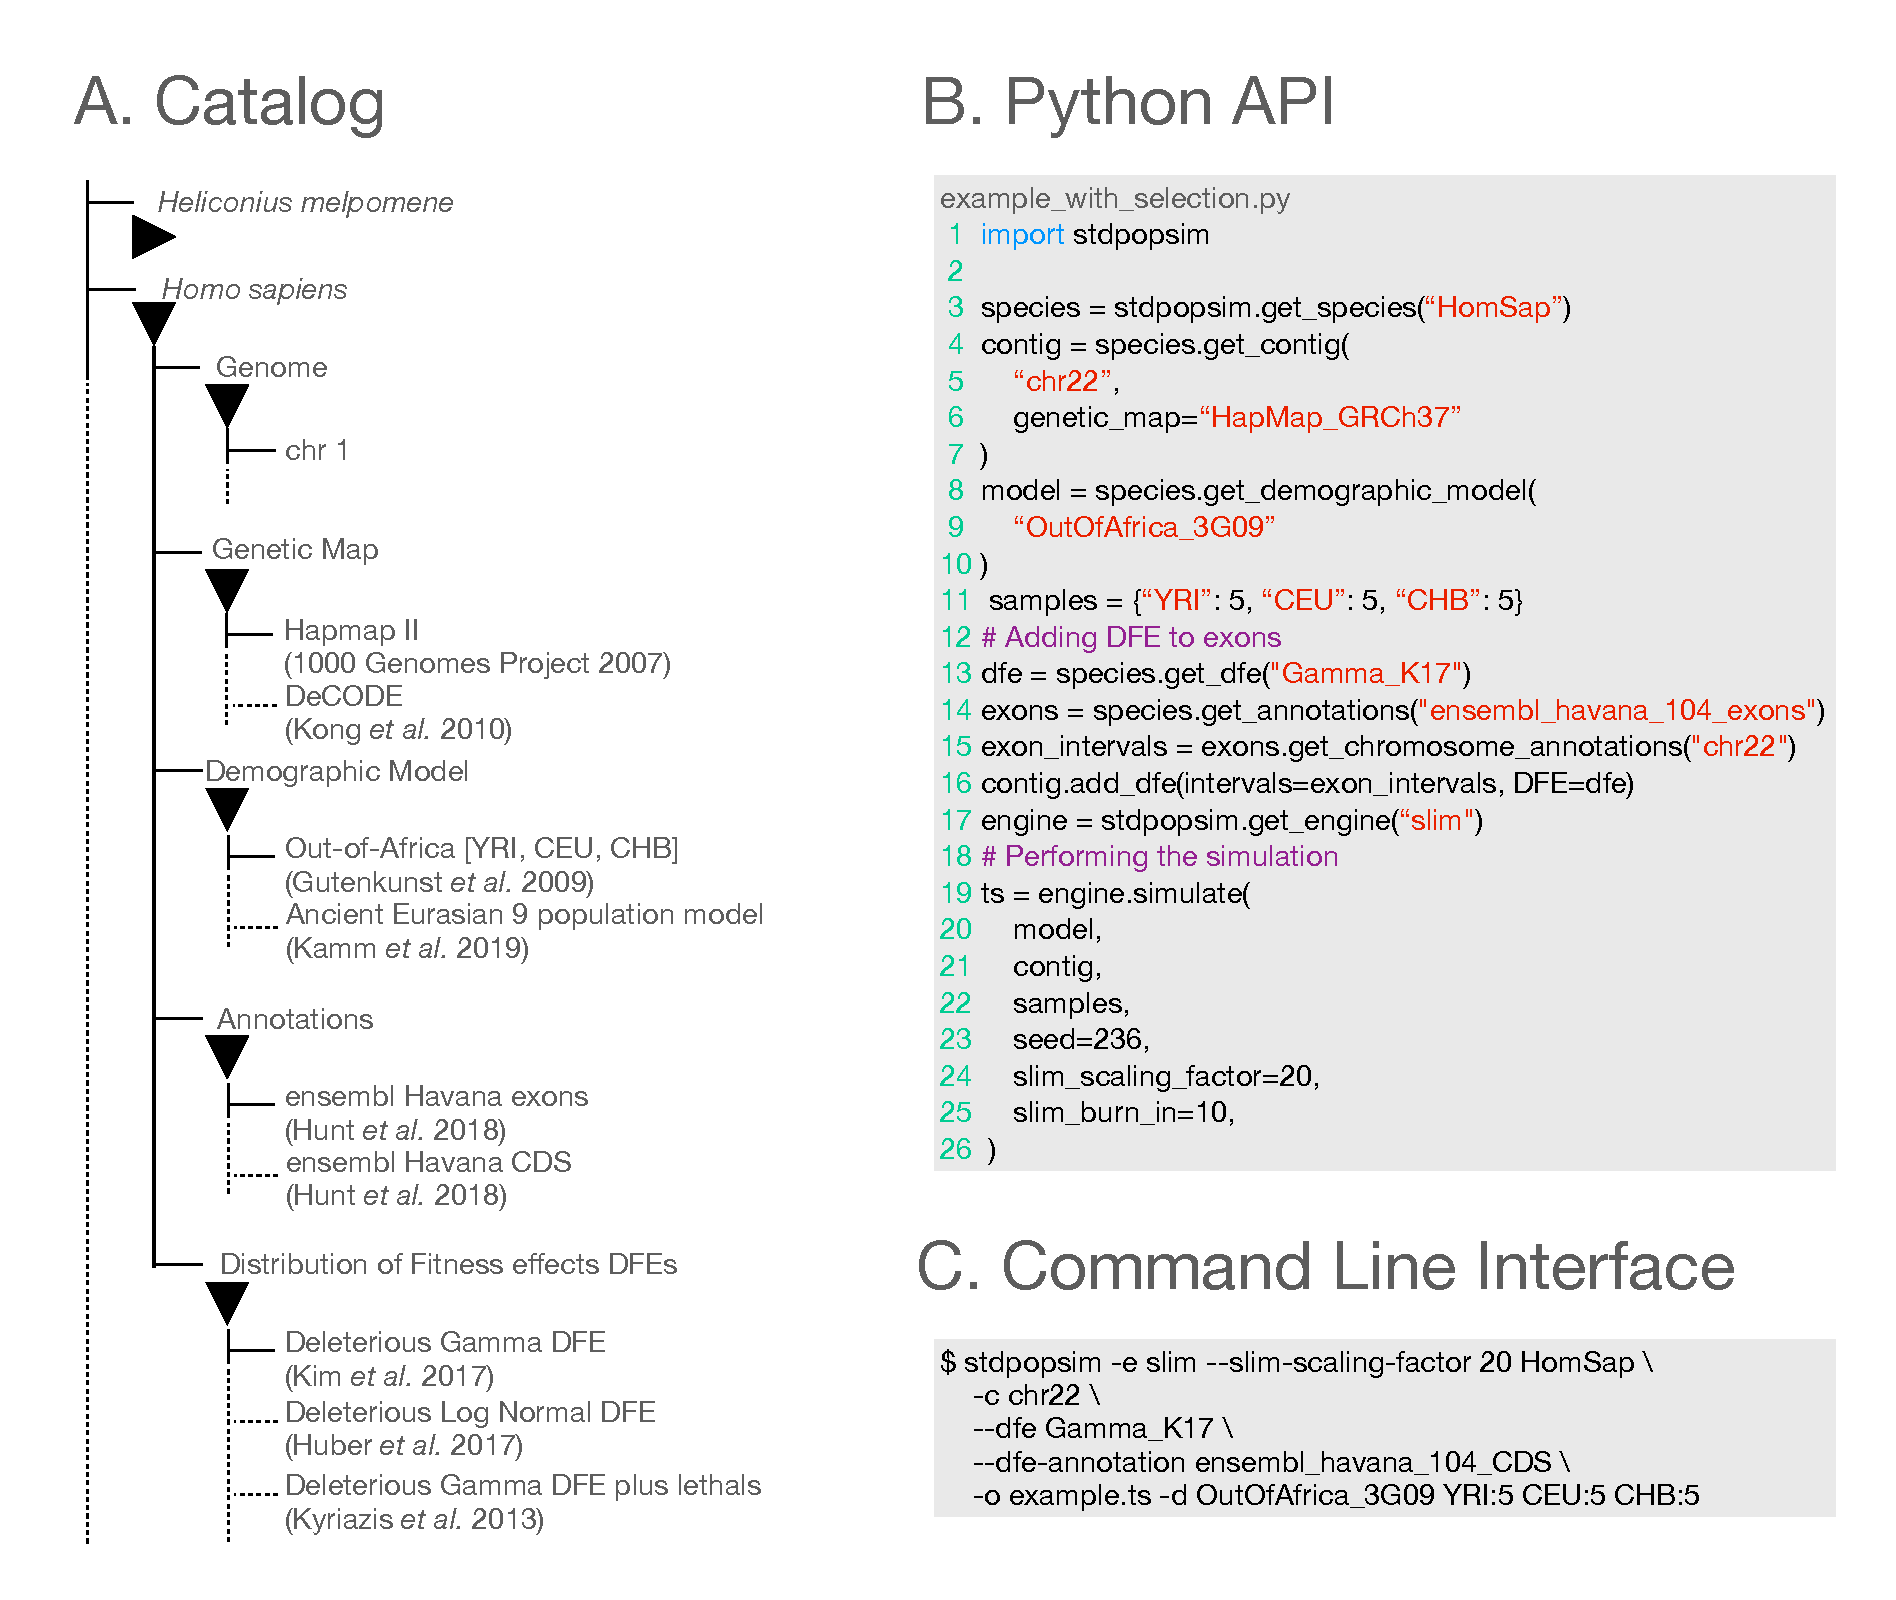
\includegraphics[width=\linewidth]{figures/schematics/catalog.pdf}
        \caption{\label{fig:schematic}
        A schematic of the \stdpopsim catalog for simulating genetic variation
        in a population. The user specifies a species, a portion of the genome to simulate,
        and optionally a genetic map, a model of demography, and a model of selection that 
        itself is composed of a distribution of fitness effects (DFE) and a set of functional
        annotations.}
    \end{wrapfigure}

    The vast majority of published DFE estimates are based on a limited number of species,
    so \stdpopsim currently has implemented published DFEs from
    four species: \textit{Arabidopsis thaleana} \citep{huber2018gene}, \textit{Drosophila melanogaster} \citep{ragsdale2016triallelic,huber2017determining},
    humans \citep{huber2017determining,kim2017inference}, and the vaquita porpoise \textit{Phocoena sinus} \citep{robinson2022critically}.
    While that is so, these DFEs can be applied to other species
    in the catalog. For instance, one could simulate a butterfly species with a gamma DFE originally
    estimated from humans, or a human population with a DFE estimated from \textit{Drosophila}.
    Furthermore the user can specify a custom DFE, and provide their own annotations
    of functional elements to simulate selection in a species for which we do not yet have 
    a published DFE included in the catalog. This flexibility allows for a wide range of
    models of selection to be simulated. %, and for the results of these simulations to be
    %compared to empirical data or used as a null model for hypothesis testing.
    % DRS: commenting that stuff out because there are obviously other use cases that could be
    % listed here (e.g. ML/ABC, and if we don't know enough about a species to do that then
    % we probably have no business doing hypothesis testing either, which could be just as
    % misleading or maybe even more so), so the simplest solution is to cut this as it is
    % not needed here.
   
    % sweep interface
    In addition to the \texttt{DFE} class, we have also implemented a class (\texttt{stdpopsim.ext.selective\_sweep})
    that enables selective sweeps to be simulated in \stdpopsim.
    This class augments a demographic model with an ``extended event''
    which conditions on the introduction of a selected mutation at a given time and position
    and with a given selection coefficient. Further the user can specify the minimum frequency
    of the selected allele at the time of sampling. As these extended events are implemented
    on top of the existing \stdpopsim API, they can be combined with other models of selection
    and demography to provide a rich model of the combined effects of multiple disparate evolutionary processes
    on genetic variation in a population.
    
    % current numbers of DFEs / species / etc
    % DRS: are we giving this a version number?
    At this release the \stdpopsim catalog comprises 24 species (i.e. genome representations)
    for which we have implemented 28 demographic models, have 37 genetic maps, and 7 DFEs. %someone should double check the numbers
    Additions to the catalog are ongoing---we point the reader to our previously published 
    report detailing this effort \citep{lauterbur2023expanding}. We welcome contributions from the
    community and encourage those interested in contributing to visit https://popsim-consortium.github.io/stdpopsim-docs
    or contact one of the PopSim Consortium members for guidance.


    
\section*{Example Applications with Selection}
    \label{applications}
    In this section we provide a series of examples of how the new models of selection
    in \stdpopsim can be used to benchmark different
    methods for population genetic inference.
    We focus on three main areas: demographic inference in the 
    single and multi-population settings, inference of the DFE,
    and the detection of selective sweeps, particularly in the context of background selection.

    \section*{Inference of $N_e(t)$ in the context of selection}
    One of the most common applications of population genetic inference is to estimate
    the effective population size over time, $N_e(t)$, from genetic data. This can be done
    using a variety of methods, including the pairwise sequentially Markovian coalescent
    (PSMC) \citep{li2011inference}, through use of the site frequency spectrum (SFS) \citep{liu2020stairway},
    as well as through identity by decent information \citep{santiago2020recent}. 
    While that is so, it has been well described that selection, because of its effects on
    patterns of genetic variation, can bias estimates of $N_e(t)$
    away from true census population sizes simply because selection increases the 
    rate of coalescence in the genome \citep[e.g.][]{schrider2016effects}. 

    Using \stdpopsim we can easily simulate genetic data under a model of selection and then 
    examine the performance of different methods for inferring $N_e(t)$ from these simulated 
    data. In Figure \ref{fig:1pop-human-demography} we show the results of such a benchmark
    where we have simulated genomes under a model of human out of Africa (OOA) demography
    with and without purifying selection on exons. For this simulation we have used
    a genetic map from the HapMap Project \citep{international2007second} along with a
    DFE for deleterious alleles (estimated by \cite{huber2017determining})
    that acts on exonic positions defined from the HAVANA group release 104 for the human genome.
    % DRS: Maybe we should say something about how easy it was to do these simulations, and maybe even show
    % some example code somewhere to prove our point? Could help emphasize the utility of this resource.
    These simulations were then used to estimate $N_e(t)$ using four methods: 1) \msmc \citep{Schiffels2020}, 
    2)\stairway method \citep{liu2020stairway}, 3) \gone \citep{santiago2020recent}, and 4) \smcpp \citep{terhorst2017robust}.
    In this and what follows we have performed 3 replicate whole genome simulations, so uncertainty in estimates might
    be roughly assessed, however we are mindful of wasted computational resources as thorough benchmarking
    isn't the main purpose of this manuscript.
    
    In Figure \ref{fig:1pop-human-demography} we show six panels, each of which shows the estimated $N_e(t)$
    from data simulated under the five-population model of human out-of-Africa demography
    from Ragsdale \textit{et al.} (2019)
    with samples taken from three modern geographic groups (CEU, CHB, and YRI from left to right).
    The top row shows the results of $N_e(t)$ estimates made from simulations without selection, while the bottom row shows the results
    from simulations with deleterious mutatinos occurring in exons.
    In each panel we show the true $N_e(t)$ in black, and the estimated $N_e(t)$
    in various colors for the four methods. Dotted lines on the bottom row are to visually reinforce that inference is done
    from a model with selection. We see that these methods generally perform reasonably well in the absence of selection, 
    although GONE seems to overestimate $N_e(t)$ in the more recent past for the CEU and CHB populations.
    Presumably this could be due to patterns of linkage disequilibrium that result from the combination
    of bottleneck and growth in these populations.
    In the presence of selection, different methods behave differently. 
    For instance stairwaiplot which uses the SFS to infer $N_e(t)$ seems to slightly underestimate $N_e(t)$
    but is reasonably close to the true $N_e(t)$ in the absence of selection.
    Likewise \smcpp seems to be more robust to the presence of selection,
    but there is some added noise to the returned estimates. 
    \msmc seems to be the most affected by the presence of selection, 
    estimates of $N_e(t)$ varying quite a bit from the true $N_e(t)$,
    although estimates from \msmc have quite a bit of added noise even in the absence of selection.

    % DRS: I don't agree with the interpretation in the previous two sentences (starting with "Likewise").
    % MSMC is already barfing a little bit even without selection, and it is not clear to me from these
    % plots that selection makes things any worse. Also, SMC++ is doing quite well without selection so maybe
    % the minor drop in accuracy is meaningful in relative terms.
    % ADK: I edited the text-- what do you think Dan?
    % DRS: I am still finding this description pretty inaccurate. Happy to discuss over zoom if you think
    % that might be faster.



    \begin{figure}[t]
        \centering
        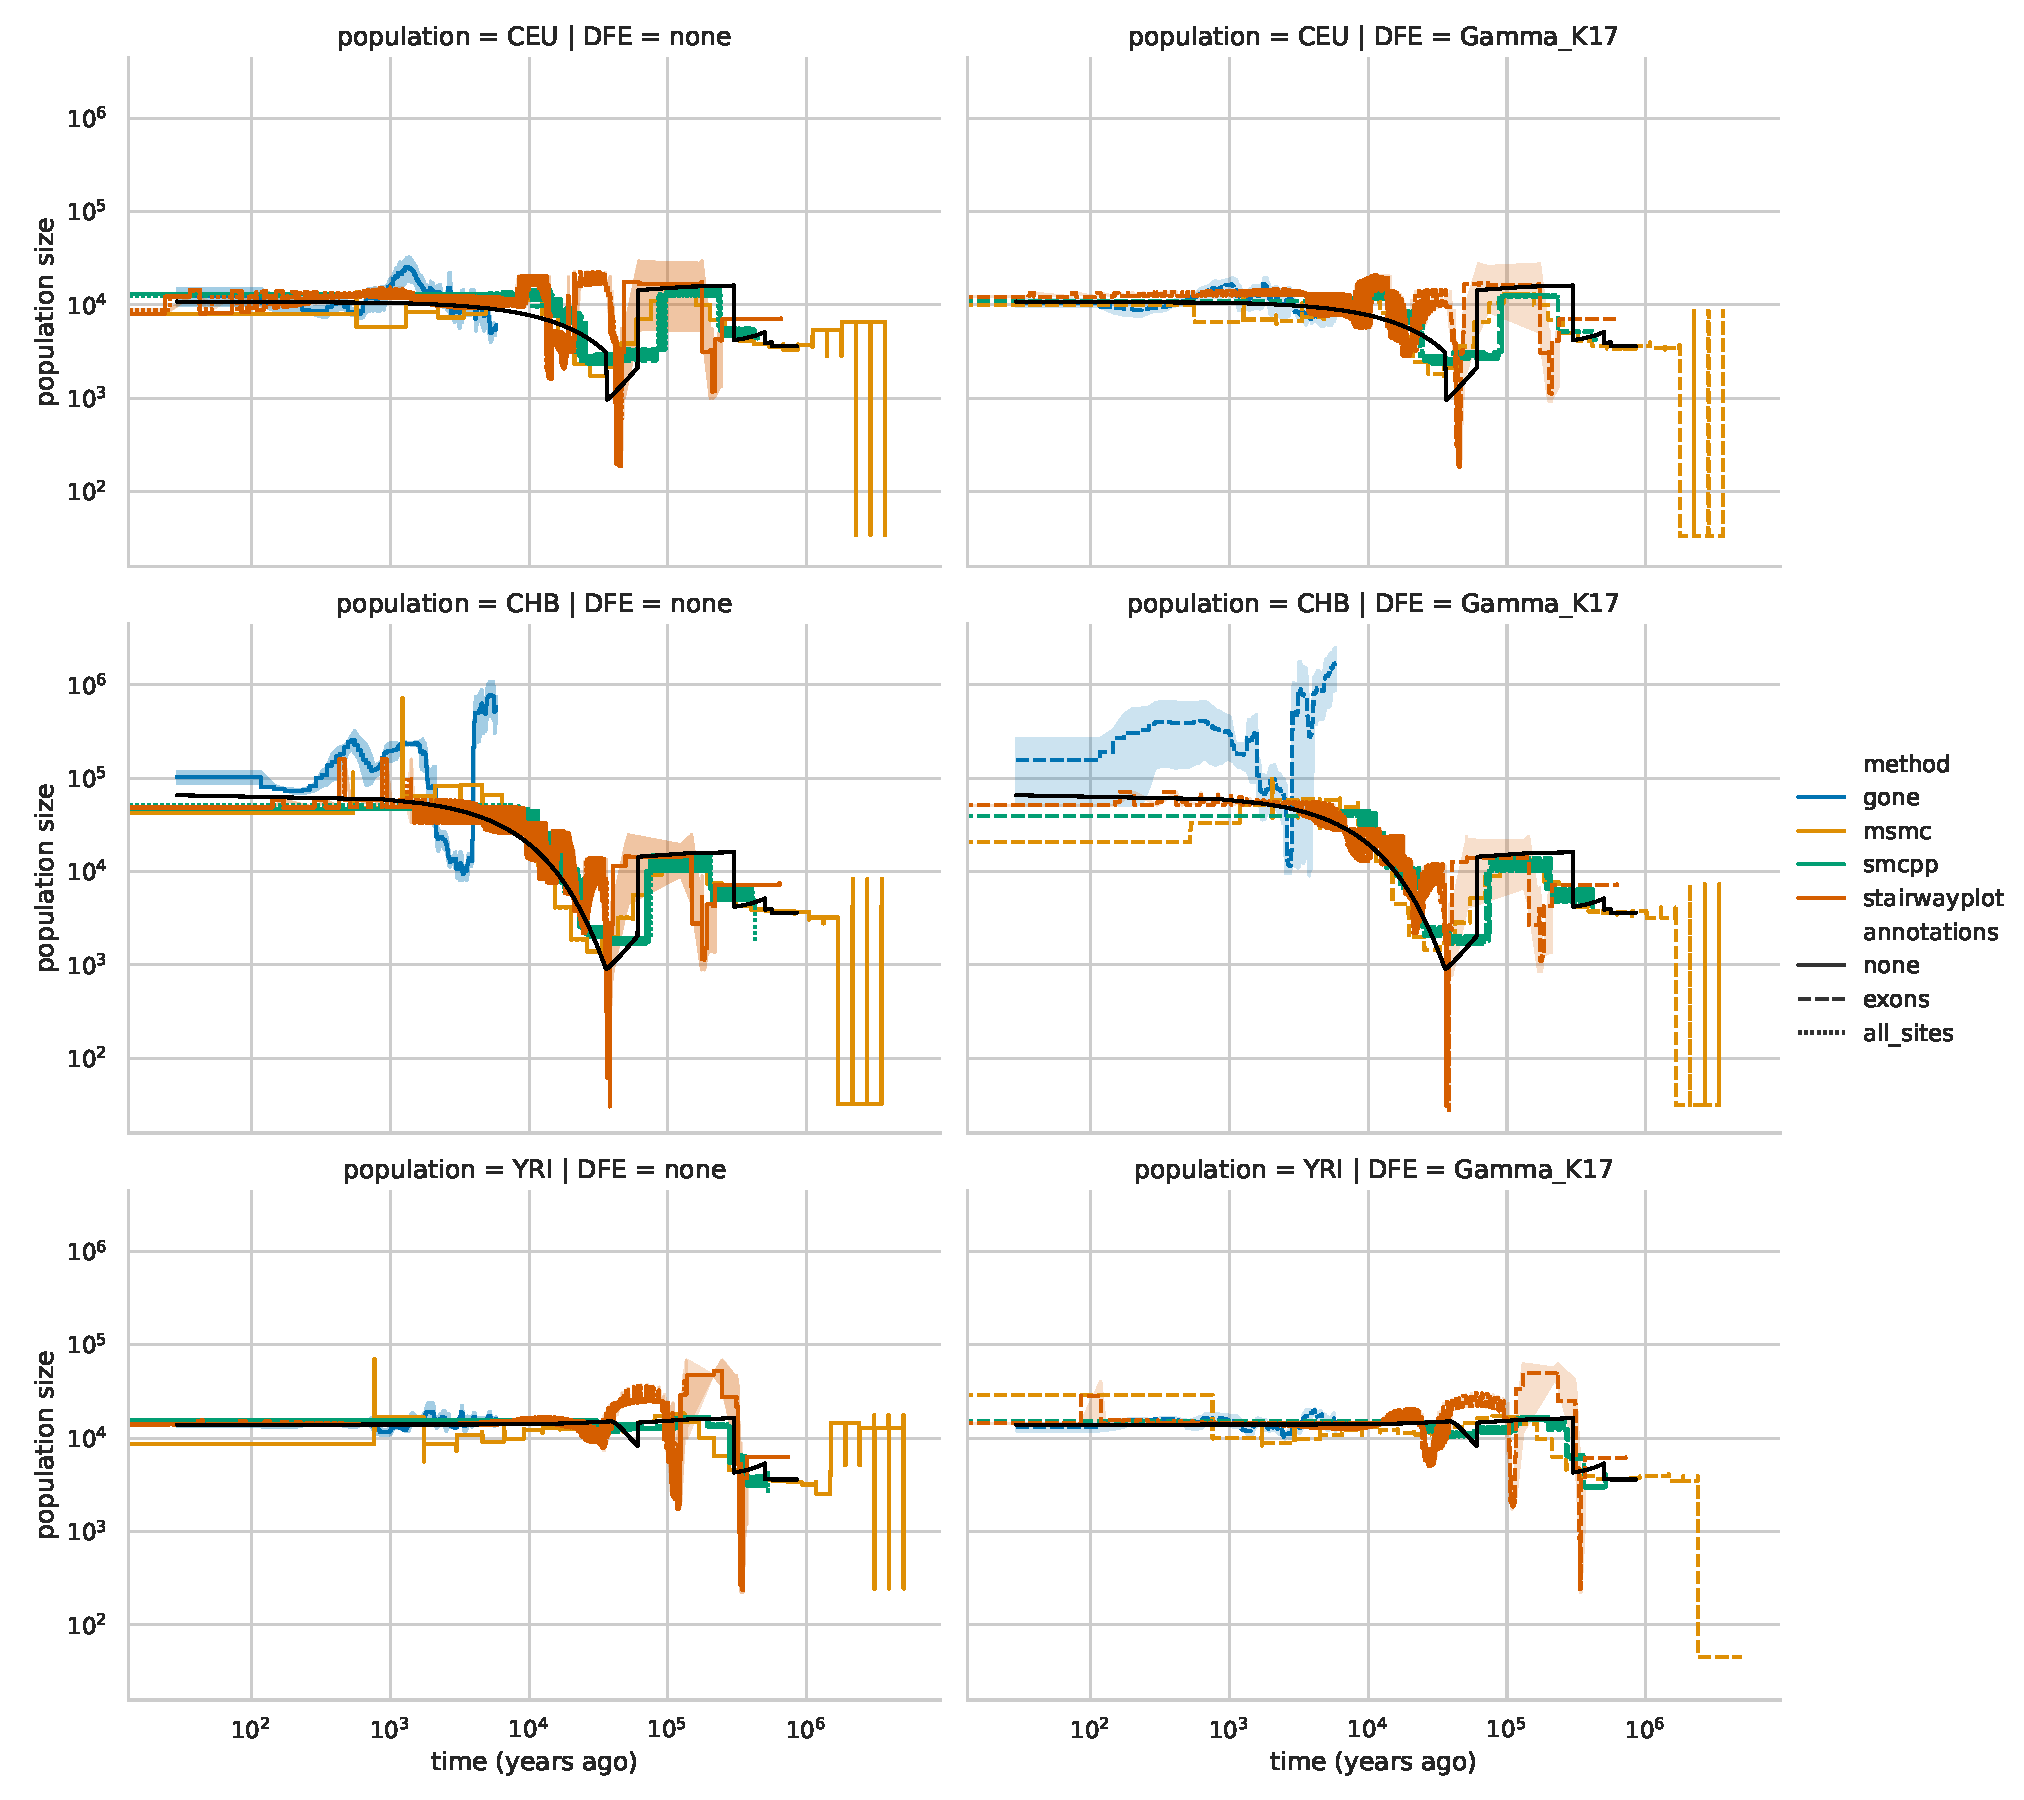
\includegraphics[width=\textwidth]{figures/HomSap/OOA/estimated_Ne_t_final}
        \caption{
        \label{fig:1pop-human-demography}
        Performance of methods to infer $N_e(t)$ from a human out-of-Africa model \citep{ragsdale2019models}
        with and without purifying selection on exons. The top row shows estimates of $N_e(t)$ from simulations
        without selection, while the bottom row shows estimates of $N_e(t)$ from simulations with a gamma-distributed   
        DFE acting on exons. In each panel we show the true $N_e(t)$ in black, and the estimated $N_e(t)$ from four methods:    
        \msmc \citep{Schiffels2020}, \stairway \citep{liu2020stairway}, \gone \citep{santiago2020recent}, and \smcpp \citep{terhorst2017robust}.  
        }
    \end{figure}
    %DRS-fig: reminder to update the legend to just say ``exons'' instead of ensembl_havana_whatever...

    To highlight the ease of comparisons between different species and models enabled by \stdpopsim,
    we have also performed a similar benchmark using the vaquita porpoise \textit{Phocoena sinus}.
    In Figure \ref{fig:1pop-vaquita-demography} we show the results of $N_e(t)$ inference
    where we have simulated genomes under a model of vaquita demography from \textcite{robinson2022critically}.
    For these simulations we have used the genome structure and exon annotations from the vaquita genome assembly
    and a DFE from \textcite{robinson2022critically} that acts on exons, however no genetic map 
    is currently available, so recombination rates are assumed to be constant across the genome.
    The demographic model is a simple two-epoch model where population size has declined in the recent past. 
    In this case we see that all methods perform well both in the absence and presence of selection,
    with a close match between the true $N_e(t)$ and the estimated $N_e(t)$ in all cases.


\begin{figure}[t]
    \centering
    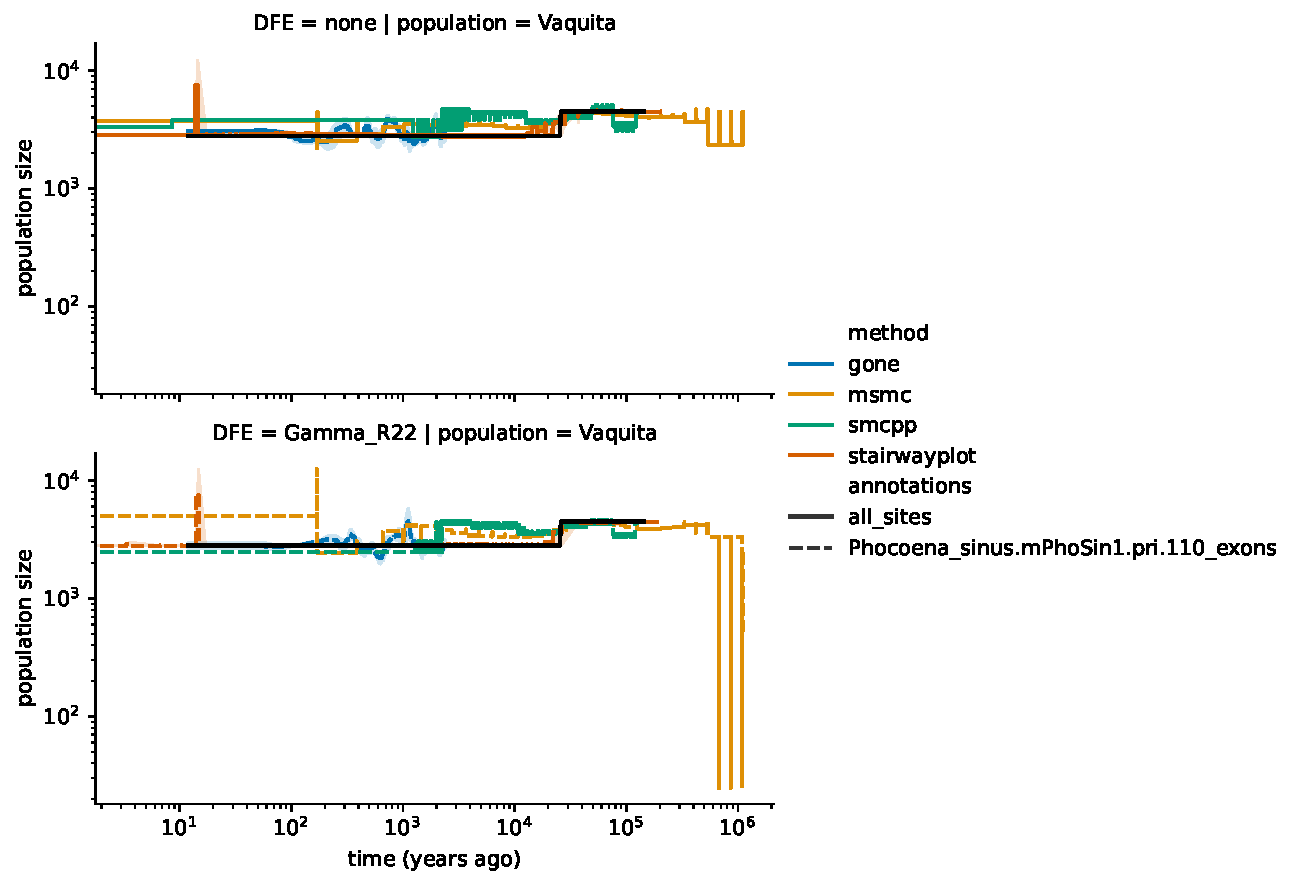
\includegraphics[width=\textwidth]{figures/PhoSin/Vaquita2Epoch_1R22/estimated_Ne_t_final}
    \caption{
    \label{fig:1pop-vaquita-demography}
    Performance of methods to infer $N_e(t)$ from simulations of the vaquita porpoise genome under a single population
    model of declining population size \citep{robinson2022critically} with and without background selection on exons. 
    The top panel shows estimates of $N_e(t)$ from simulations
    without selection, while the bottom panel shows estimates of $N_e(t)$ from simulations with a gamma-distributed   
    DFE acting on exons. In each panel we show the true $N_e(t)$ in black, and the estimated $N_e(t)$ from four methods:    
    \msmc \citep{Schiffels2020}, \stairway \citep{liu2020stairway}, \gone \citep{santiago2020recent}, and \smcpp \citep{terhorst2017robust}.  
    }
\end{figure}

\section*{Estimation of the Distribution of Fitness effects}
    \label{dfe}
    Another common application of population genetic inference is to estimate the distribution of fitness effects (DFE)
    from genetic data. Here we show how the new models of selection in \stdpopsim can be used to benchmark and compare
    the performance of different methods for inferring the DFE. We performed simulations using the 
    human and vaquita porpoise models described above, with complex demographic histories and models of selection acting on exons.

    \begin{figure}[htbp]
        \centering
        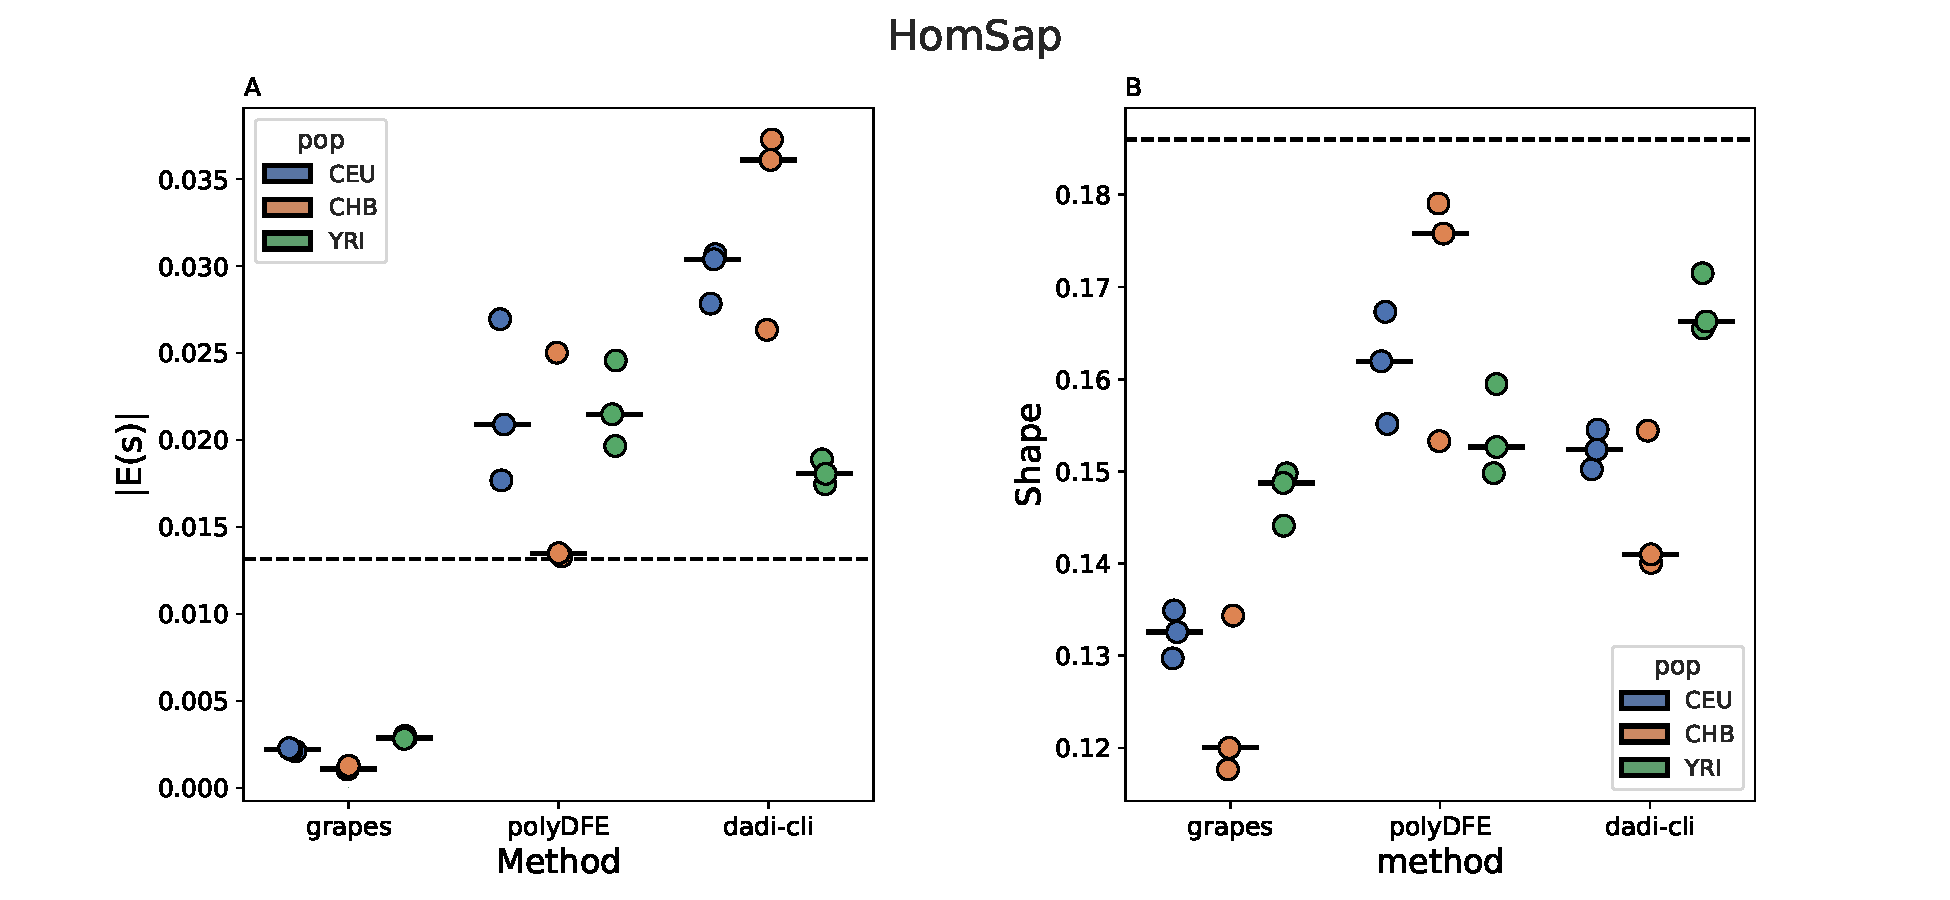
\includegraphics[width=\linewidth]{figures/HomSap/OOA/HomSap_OutOfAfricaArchaicAdmixture_5R19_Gamma_K17_ensembl_havana_104_exons_DFE_plot}
        \caption{A comparison of methods for inferring the distribution of fitness effects (DFE) from genetic data.
        Simulations were performed using a human out-of-Africa model \citep{ragsdale2019models} with a gamma-distributed DFE
        acting on exons parameterized by a mean selection coefficient and a shape parameter. Estimates of the 
        parameters of the DFE are shown in the left ($\lvert E(s) \rvert $) and right hand panels (shape) respectively.
        The human model has three extant populations (CEU, CHB, and YRI), and parameter estimates from each
        sample are shown in different colors.
        Estimates from three different methods are shown: 1) \grapes \cite{galtier2016adaptive}, 2) \polydfe \citep{tataru2020polydfe},
        and 3) \dadi \citep{gutenkunst2009inferring}.}
        \label{fig:homsap-dfe.ooa}
    \end{figure}

    In Figures \ref{fig:homsap-dfe.constant} and \ref{fig:homsap-dfe.ooa} we show a comparison of estimates
    from three software packages for inferring the DFE from genetic data:
    \dadi \citep{gutenkunst2009inferring}, \polydfe \citep{tataru2020polydfe}, 
    and \grapes \citep{galtier2016adaptive}.
    In each case we note that the DFE is estimated from segregating sites only,
    without the use of substitution data, as a current limitation of \stdpopsim
    currently is that we are not able to simulate an outgroup sequence to estimate
    divergence. 
    Figure \ref{fig:homsap-dfe.constant} shows estimates from a single, constant size population of humans, 
    while Figure \ref{fig:homsap-dfe.ooa} shows estimates from a model of human out-of-Africa demography.
    In a constant size population, all methods perform reasonably well, although \dadi seems to
    perform slightly worse than the other methods examined, at least for the small number of replicates we simulated here.
    Notably only \polydfe overlapped the true mean selection coefficient, whereas 
    the other methods slightly underestimated the strength of selection. 
    For the shape parameter in constant size simulations \grapes and \polydfe are roughly
    equivalent in their performance whereas \dadi seems to yield overestimates. 
    
    In the out-of-Africa model (fig \ref{fig:homsap-dfe.ooa}) the performance of the methods is more mixed. 
    In particular variation in accuracy of the parameters estimated in each
    sample population depends on the methods used, and each method seems to 
    have its own biases with respect to the way in which population history 
    affects parameter estimates. For instance for \dadi we see that estimates of 
    the shape parameter are most accurate in the YRI sample, while for \polydfe
    estimates are least accurate in the YRI sample. 
    With respect to the strength of selection, as in constant size populations,
    all methods are performing reasonably well, although \dadi seems to
    trail in terms of accuracy.


    %add PhoSin DFE figure here
    \begin{figure}
        \centering
        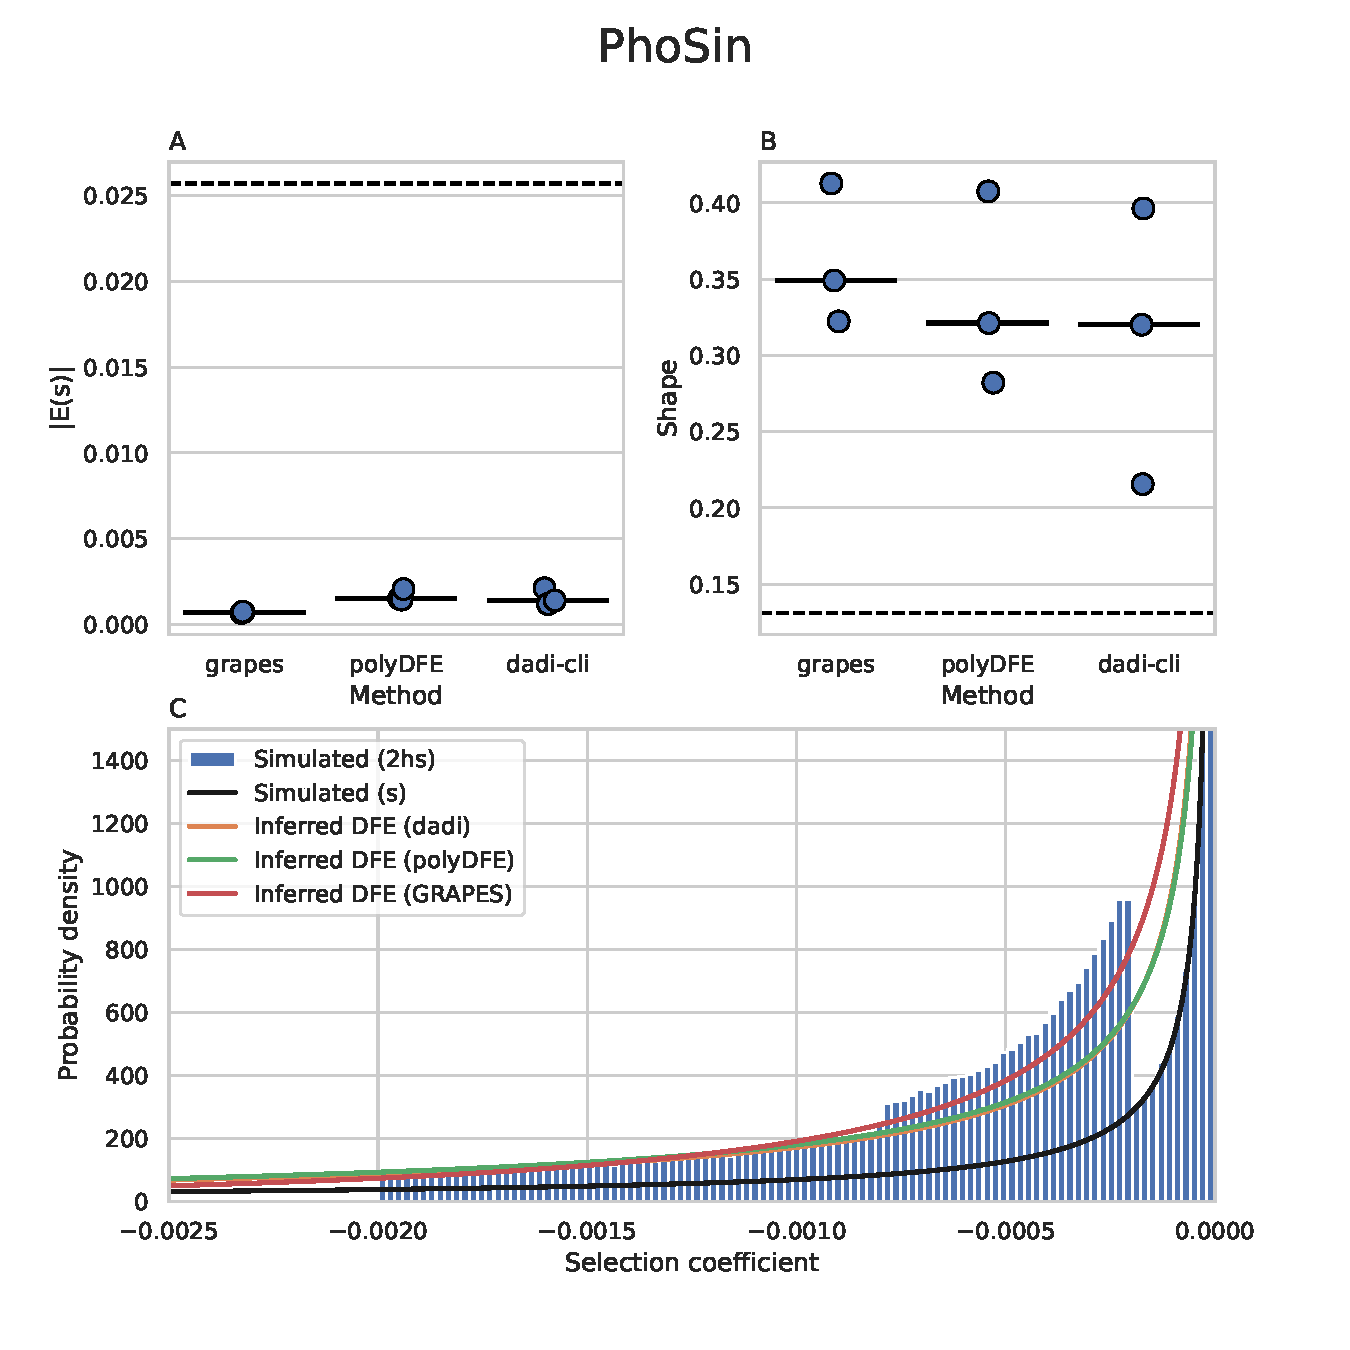
\includegraphics[width=0.8\textwidth]{figures/PhoSin/Vaquita2Epoch_1R22/PhoSin_Vaquita2Epoch_1R22_Gamma_R22_Phocoena_sinus.mPhoSin1.pri.110_exons_DFE_plot.pdf}
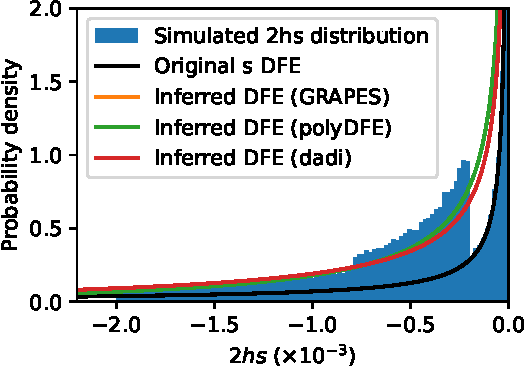
\includegraphics{figures/PhoSin/Vaquita2Epoch_1R22/hs_hist.pdf}
        \caption{
        \label{fig:vaquita-dfe}
        A comparison of methods for inferring the distribution of fitness effects (DFE) from genetic data.
        Simulations were performed using a model of vaquita porpoise demography \citep{robinson2022critically} with a gamma-distributed DFE
        acting on exons parameterized by a mean selection coefficient, a shape parameter, and a relationship between selection and domiance. Estimates of the 
        parameters of the DFE are shown in the left ($\lvert E(s) \rvert $) and right hand panels (shape) respectively.
        This vaquita model has a single extant population, and parameter estimates from each
        of the three different methods are shown: 1) \grapes \cite{galtier2016adaptive}, 2) \polydfe \citep{tataru2020polydfe},
        and 3) \dadi \citep{gutenkunst2009inferring,kim2017inference}.
        C) Shown is the simulated distribution of $2 h s$, where $h$ is the dominance coefficient, along with the simulated distribution of $s$ and the median inferred DFEs. The distribution of $2 h s$ is multimodal because the simulated relationship between $h$ and $s$ is not continuous.
        % RNG: For C, need to extract inferred values from pipeline.
        }
    \end{figure}
    
    In Figures \ref{fig:vaquita-dfe.constant} and \ref{fig:vaquita-dfe} we show a comparison of estimates
    from the same three DFE-inference packages on simulations of the
    vaquita porpoise genome. In the constant size model (fig \ref{fig:vaquita-dfe.constant}) we see that all methods
    perform uniformly worse that in the human genome simulations, with consistent underestimation of the mean selection coefficient    
    and overestimation of the shape parameter. 
    A critical distinction is that the previous human simulations employed a DFE that assumed all selected mutations had additive effects
    (no dominance, $h = 1/2$), whereas the vaquita simulations use a DFE in which more deleterious mutations are more recessive ($h < 1/2$).
    For all three software packages, the inferred mean and shape of the distribution of selection coefficients 
    is consistent with the mean and shape of the distribution of $2 h s$, the product of the dominance coefficient
    and the selection coefficient (Fig.~\ref{fig:vaquita-dfe}C).
    This is likely because deleterious alleles are typically at low frequency and thus heterozygous, 
    where their selective effect is $h s$, and all these tools assume additivity  ($h = 1/2$).
    Strongly deleterious alleles are often observed to be recessive in many species \citep{mukai1972mutation},
    so these results suggest caution in interpreting DFE inferences.
    %RNG: Could use Kirk's help with the best references here

\section*{Detection of Selective Sweeps}
    \label{sweeps}
    We next highlight how the new models of selection in \stdpopsim can be used to benchmark and compare
    the performance of different methods for detecting selective sweeps from genetic data. 
    Here we have performed simulations of human chromosome 1 under the three population out-of-Africa model from \cite{gutenkunst2009inferring}
    with purifying selection acting on exons under the gamma-distributed DFE described above, the HapMap II genetic map \citep{international2007second},    
    but also include sweeps. In particular we introduced a beneficial mutation
    at a given location (to be varied) in the genome at a given time, and with a moderately strong selection coefficient ($s = 0.03$; $2Ns \sim 600$).
    For each sweep location we performed 200 replicate simulations, sampling from them only if the selected allele reached a frequency of
    0.95 or greater. Rather than simulate the entire chromosome arm, replicate simulations were performed on 5cM regions of the chromosome
    at each of 100 different locations. As recombination rate varies across the genome, the size of the region in base pairs simulated varies,
    however the recombination distance, which is critical for the linked effects of a sweep, is held constant.
  

    %sweeep power figure
    \begin{figure}
        \centering
        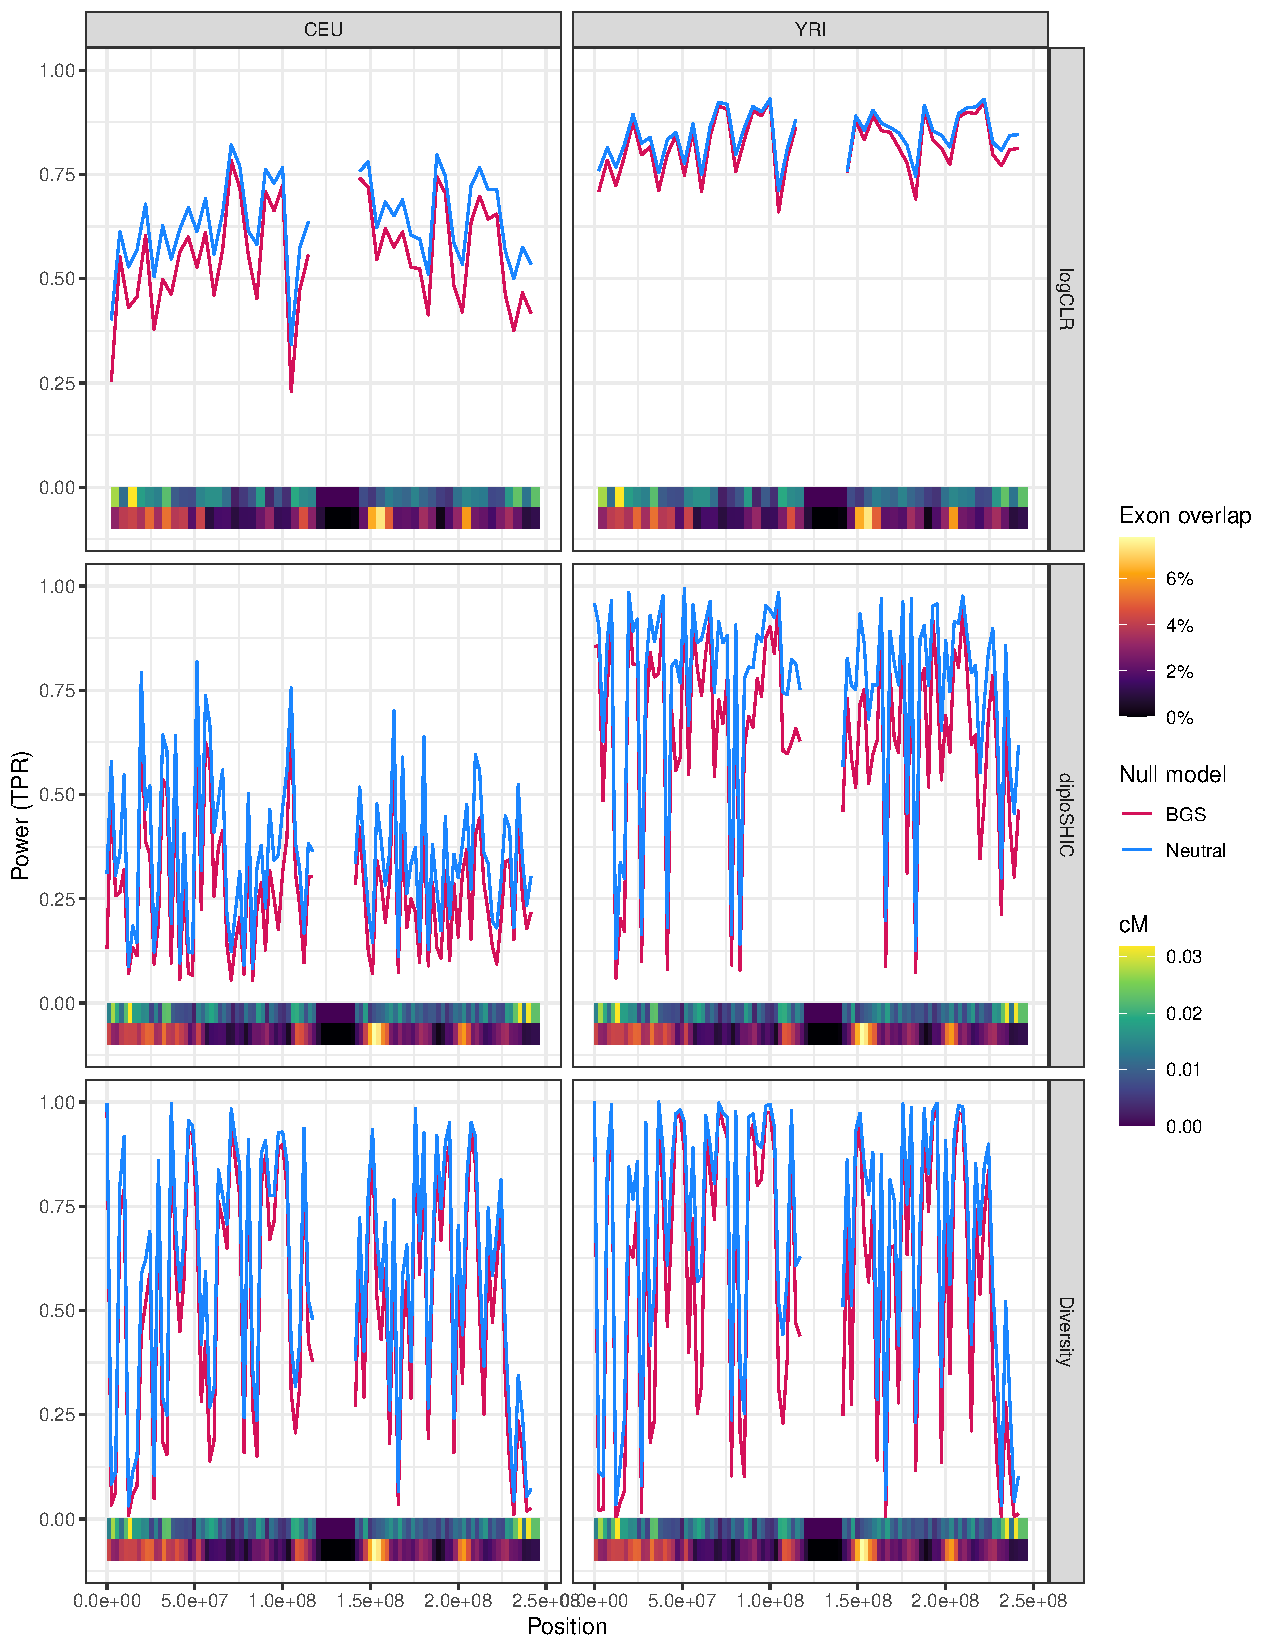
\includegraphics[width=0.8 \textwidth]{figures/sweeps/chr1_power.pdf}
        \caption{
        Power to detect selective sweeps at 100 locations along human chromosome 1 under a three population out-of-Africa model \citep{gutenkunst2009inferring}  
        with and without purifying selection acting on exons under the gamma-distributed DFE described above. 
        The HapMap II genetic map \citep{international2007second} was used in each simulation. 
        Single beneficial mutations were introduced at each location with a selection coefficient of $s = 0.03$,
        and only sampled if they reached a terminal frequency of 0.95 or greater. 
        Three methods for detecting sweeps were used: 1) \sweepfinder \citep{degiorgio2016sweepfinder2} (top row), 
        2) \diploshic \citep{kern2018diplos} (middle row), and 3) an empirical cutoff of $\pi$ to find regions of reduced diversity (bottom row).
        True positive rate is shown for these methods for the CEU and YRI samples (left and right respectively). 
        Under each method we show heatmaps of exon density and local recombination rate along the chromosome.
        Power is shown as the proportion of replicates in which a sweep was detected at each location. 
        Each panel shows the results of simulations with purifying selection acting on exons (red; labelled BGS)
        and without purifying selection acting on exons (blue; labelled Neutral).
        }
        \label{fig:chr1_power}
    \end{figure}
    
    In Figure \ref{fig:chr1_power} we show the power to detect selective sweeps at 100 locations along human chromosome 1 from
    the simulations described above. We show the results of three methods for detecting sweeps: 1) \sweepfinder \citep{degiorgio2016sweepfinder2},
    2) \diploshic \citep{kern2018diplos}, and 3) an empirical cutoff of $\pi$ to find regions of reduced diversity.
    A few things are immediately apparent from this figure. First, the power to detect sweeps is generally higher in the YRI sample
    than in the CEU sample, which is consistent with the fact that the YRI sample has a larger effective population size and thus both stronger selection and
    more variation to detect a sweep. Further the population size of YRI has been relatively constant over the last 100,000 years,
    thus the out-of-Africa bottleneck has does not mute the signal of a sweep as much as in the CEU sample. This is consistent with
    what we know about the effects of demography on the power to detect sweeps \citep[e.g.,][]{simonsen1995properties}.
    Second, the power to detect sweeps is slightly lower in the presence of purifying selection acting on exons (consistent with \cite{schrider2020background}) but the effect is not
    as strong as one might expect. This is likely because the strength of selection acting on exons is relatively weak, and the
    sweep detection methods we have used are relatively robust to the effects of background selection. 
    Finally and most importantly, the power to detect sweeps varies considerably among regions of the genome. 
    Indeed variation in power along the chromosome is much greater than the variation in power between the CEU and YRI samples or between
    models with or without purifying selection. This is likely due to the effects of recombination rate heterogeniety as well
    as the density of functional elements along the chromosome.

    Using this set of simulations we can also compare the power of different methods to detect sweeps.
    In general, the power of the methods varies with respect to the population history of the sample.
    For instance \sweepfinder2 has marginally higher power to detect sweeps in the CEU sample than \diploshic,
    likely as a results of the fact that we here trained \diploshic on simulations under a constant size population,
    while the population size history of CEU is characterized by a strong recent bottleneck.
    Conversely, \diploshic has higher power to detect sweeps in the YRI sample than \sweepfinder2,
    likely because that population size history more closely matches the population size history used to train \diploshic.
    We can further explore the performance of the methods by plotting the receiver operating characteristic (ROC) curves for the methods.
    In Figure \ref{fig:roc-curves} we show the ROC curves for the three methods for detecting sweeps.
    False positive rates were established using neutral simulations that contained no sweeps
    but were conditioned on the same population history as the CEU and YRI samples.
    These suggest that the $\pi$ cutoff is a suprisingly effective method for detecting sweeps,
    in these genomic regions at least, but that it lags behind \diploshic and \sweepfinder2 in terms of specificity
    generally.
    % DRS: the ROC curve doesn't tell us which methods have better/worse specificity, just how their sensitivities compare at a given specificity
    % DRS: but we could say something about how pi might be "less robust to heterogeneity in mapping/genotyping quality across the genome than the other methods"
    % DRS: or something like that. I know we didn't test that, but it must be the case.
    %While this is not exhaustive benchmarking, we aim to give a sense to the reader
    %of how \stdpopsim can be used to benchmark the performance of different methods easily and efficiently.


    \begin{figure}
        \centering
        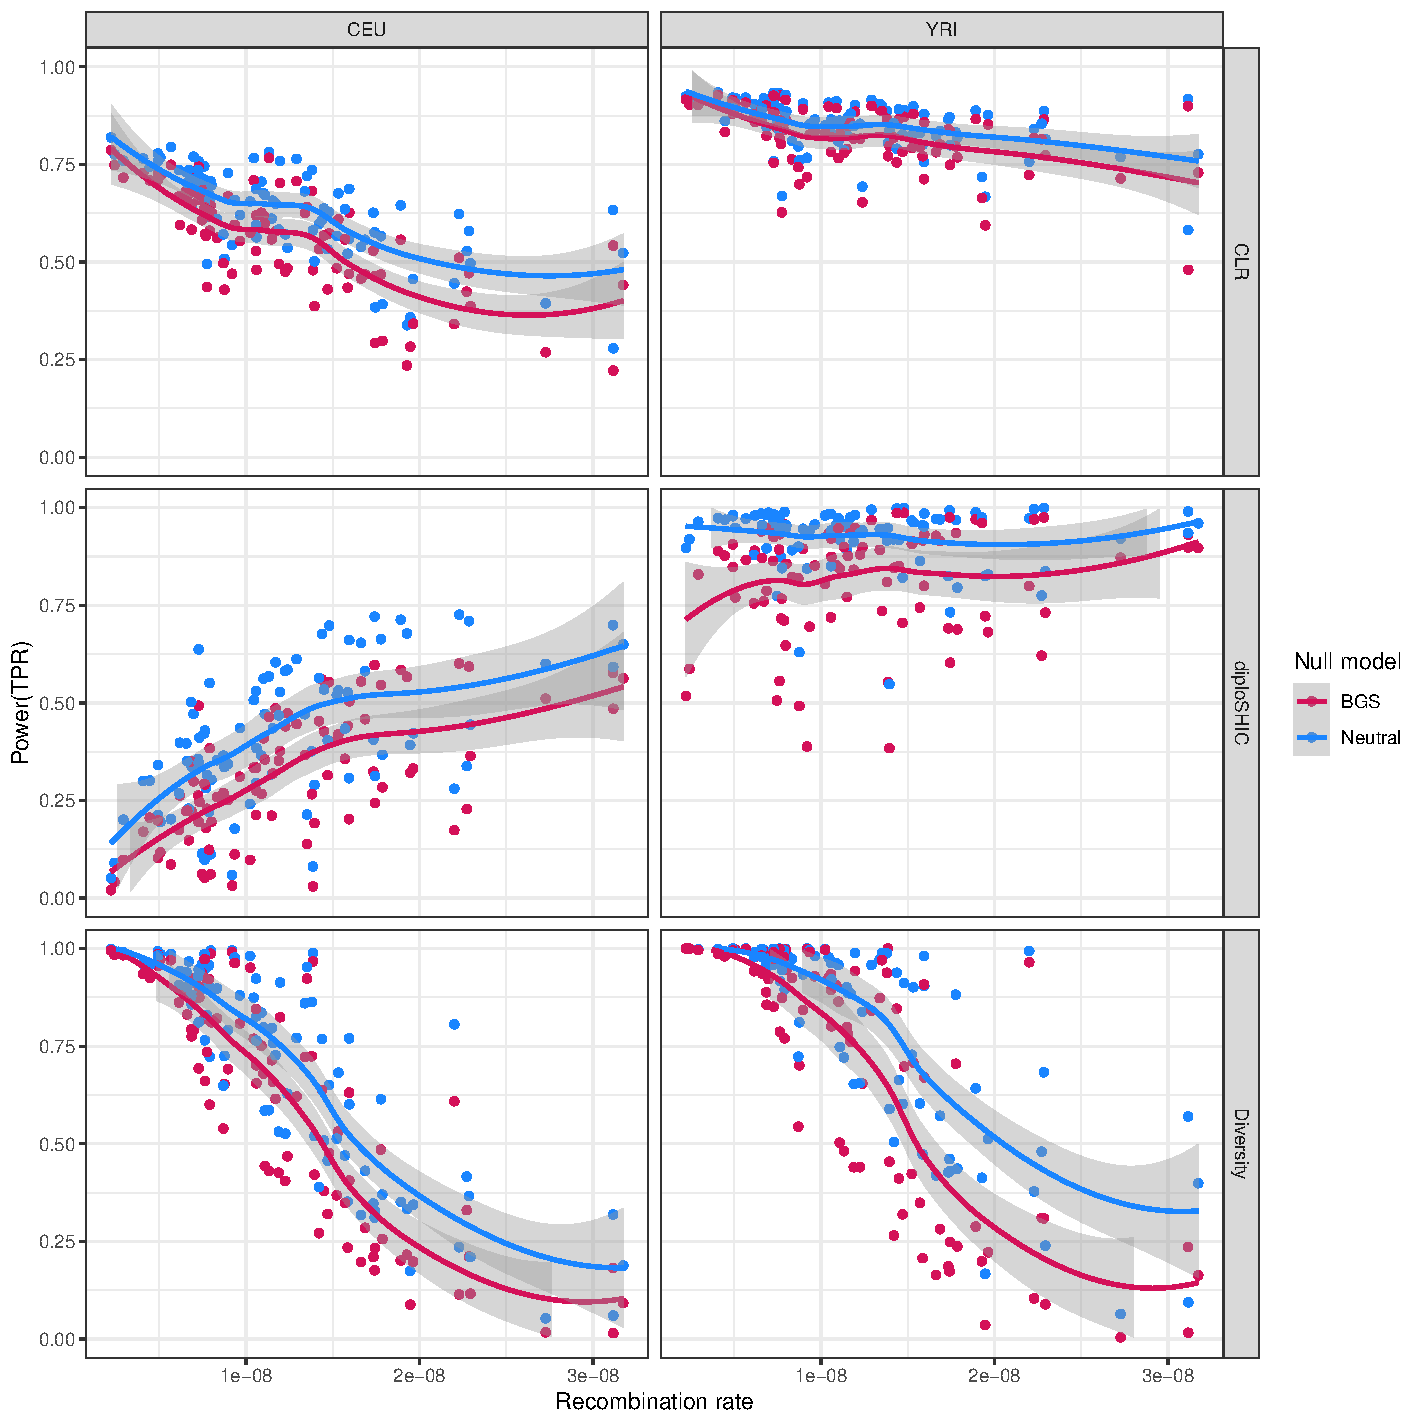
\includegraphics[width=0.8 \textwidth]{figures/sweeps/relationship_power_cM.pdf}
        \caption{
        Power to detect selective sweeps at 100 locations along human chromosome 1 under a three population out-of-Africa model \citep{gutenkunst2009inferring}  
        with and without purifying selection as a function of local recombination rate.
        Simulations are as described in Figure \ref{fig:chr1_power}.
        Each panel shows the results of simulations with purifying selection acting on exons (red; labelled BGS)
        and without purifying selection acting on exons (blue; labelled Neutral).
        True positive rate is shown for these methods for samples from the CEU and YRI samples (left and right respectively).
        Points represent the power at each location and trend lines along with 95\% confidence intervals are shown fit to those points.
        }
        \label{fig:power-recomb}
    \end{figure}

    To further explore the effects of recombination rate and exon density on the power to detect sweeps, we show in Figure \ref{fig:power-recomb}
    the relationship between power and local recombination rate for our sweep simulations. We see that power to detect sweeps is
    a decreasing function of local recombination rate for \sweepfinder2 and $pi$ outliers,
    which is consistent with sweeps having a larger genomic footprint in regions of low
    recombination.
    \diploshic on the other hand shows a slight increase in power with recombination rates.
    We also see that the presence of purifying selection acting on exons has a relatively small effect on the power to detect sweeps,    
    but one that is present across the entire range of recombinations rates observed in human chromosome 1. 
    Unsurprisingly, the empirical cutoff of $\pi$ to detect sweeps is the less robust to the effects of recombination rate than the other two methods,
    which are specifically designed to find selective sweeps. 

    In Figure \ref{fig:power-exon} we show the relationship between power and local exon density for our sweep simulations.
    Here there is little relationship between power and exon density, which is somewhat surprising given that the power to detect sweeps
    is generally lower in the presence of purifying selection acting on exons. However while this is the case we see that 
    generally all methods have more power to detect sweeps in regions of lower exon density, which is consistent with the idea that
    background selection acting on nearby exons can reduce the signature of a sweep. However this is far from a simple pattern:
    for instance sweepfinder2 seems to have minimum power in regions of intermediate exon density, while \diploshic is roughly constant
    or perhaps has a slight increase in power at intermediate exon densities. Noise in the estimates of power with respect to exon density
    are prohibitively high for the empirical cutoff of $\pi$ to detect sweeps, so it's not clear what conclusions can be drawn.
    % DRS: the exon-density results look pretty freakin flat to me. I think we could just curtail the description in this paragraph and
    % DRS: say that there are no obvious patterns that stand out from the noise?

\section*{Discussion}
    \label{Discussion}
    In this paper we have presented an important new additional to the \stdpopsim{} library
    that allows for simulating genetic variation in the presence of selection.
    We have demonstrated the utility of this new API by showing how it can be used to benchmark
    the performance of different methods for demographic inference, the inference of the distribution
    of fitness effects of mutations, and the detection of selective sweeps.
    In general, this is an important step forward for the field of population genetics,
    as it allows for a wide range of models of selection to be easily simulated and compared to
    empirical data, with reproducibility, computational efficiency, and rigor.

    We have shown how the new API can be used to benchmark the performance of different methods
    although the benchmarks shown here merely scratch the surface of what
    can be done with the new API. We envision moving forward that many researchers will use
    the new API to simulate data under a wide range of models of selection, and to develop
    new methods for the analysis of genetic data in the presence of selection. 
    The additions to \stdpopsim described here further expand this tool's utility for both 
    characterizing the patterns of diversity expected under a wide range of population genetic
    models, and for benchmarking methods for the analysis of genetic data
    on common ground
    %, using the same simulations and parameterizations of models of selection
    % DRS: this sentence got pretty bloated with my edits so I commented part of it out
    in a way that was not possible before.

\section*{Methods}
    \label{methods}

    \subsection*{Simulations}
    In this study we performed simulations of the human and vaquita porpoise genomes
    using the \stdpopsim{} framework. As stated above, simulations included a model 
    of selection acting on exonic regions, matched to the human and vaquita porpoise genomes.
    Three replicates of whole-genome simulations were performed for each species, with 
    a sample size of 100 diploid individuals. Demographic models are as stated above, each
    using the exon annotations from the human and vaquita porpoise genomes respectively.
    For simulations with selection, a SLiM scaling factor of 1 (corresponding to no scaling)
    was used, with a burn-in of 10 ticks. 

    \subsection*{Demographic inference}
    We assessed the accuracy of demographic inferences from
    \msmc \citep{Schiffels2020}, \stairway \citep{liu2020stairway}, \gone \citep{santiago2020recent}, and \smcpp \citep{terhorst2017robust}.
    Each of these methods was run using the same set of simulations in replicate.
    In each case, the non-recombining portion
    of the genome was masked to remove any bias due to recombination rate % DRS: might need more detail here
    variation. Comparisons between inferences made with and without selection were 
    of particular interest. For \msmc, we used a random sample of $N=6$ genomes with 20
    iterations of the EM algorithm. For \gone, we set max\_snps to 500000,
    the number of generations to 2000, and the number of bins to 400, all representing default settings.
    

    \subsection*{Distribution of fitness effects inference}
    We used three software packages to infer the distribution of fitness effects (DFE) from genetic data:
    \dadi \citep{gutenkunst2009inferring,kim2017inference}, \polydfe \citep{tataru2020polydfe}, and \grapes \citep{galtier2016adaptive}.
    Each software package was run using the same set of simulations.
    For these analyses we used the exon annotations from the human and vaquita porpoise genomes respectively.
    A key distinction between our analyses and those done in practice
    is that we have complete knowledge of which sites are under selection in the simulation,
    thus our inferences is a best case scenario. Empirical inference of the DFE is a much
    harder problem as some mutations assumed to be free of selection
    may in reality be under selection. As above, all methods were run using default settings.

    \subsection*{Selective sweeps detection}
    We ran simulations of 5Mbp regions of chromosome 1 of the human genome with and without
    purifying selection acting on exonic regions, and under a three population
    out-of-Africa model of human demography \citep{gutenkunst2009inferring}, 
    along with the HapMap II genetic map \citep{international2007second}.
    Single beneficial mutations were introduced at each location with a selection coefficient of $s = 0.03$,
    and only sampled if they reached a terminal frequency of 0.95 or greater. 
    We then benchmarked the performance of three methods for detecting sweeps: 1) \sweepfinder \citep{degiorgio2016sweepfinder2},
    2) \diploshic \citep{kern2018diplos}, and 3) an empirical cutoff of $\pi$ to find regions of reduced diversity.
    \diploshic was trained on data simulated using \texttt{discoal} \citep{kern2016discoal}.
    For training simulations, we simulated 20 haploid genomic regions of 1.21Mbp
    with a constant population size of 10,000 individuals, a mutation rate of 1e-8, and a recombination rate of 1e-8.
    For \texttt{discoal} simulations that included selective sweeps,
    selection coefficients were drawn from a uniform distribution between 0.001 and 0.05.
    The time of the sweep was chosen from a uniform distribution between 0 and 0.02 Ne generations in the past.
    For soft sweeps, the frequency at which selection was introduced was drawn from a uniform distribution between 1e-4 and 0.1.
    All \texttt{discoal} training simulations were done under a model of equilibrium population size, 
    so we expected it to perform suboptimally given the variation in population size in the out-of-Africa model. 

\section*{Data availability}\label{data_availability}


\section*{Acknowledgments}\label{acknowledgements}

\section*{Funding}
    \label{funding}
    Multiple funding sources supported this work.
    MFR, ST, NP, and ADK were supported in part by NIH award R35GM148253.
    %other funding sources?
\printbibliography

%%%%%%%% supplementary material
\clearpage
\beginsupplement

\section*{Supplementary Material}

% constant size DFE figure
\begin{figure}[h]
    \centering
    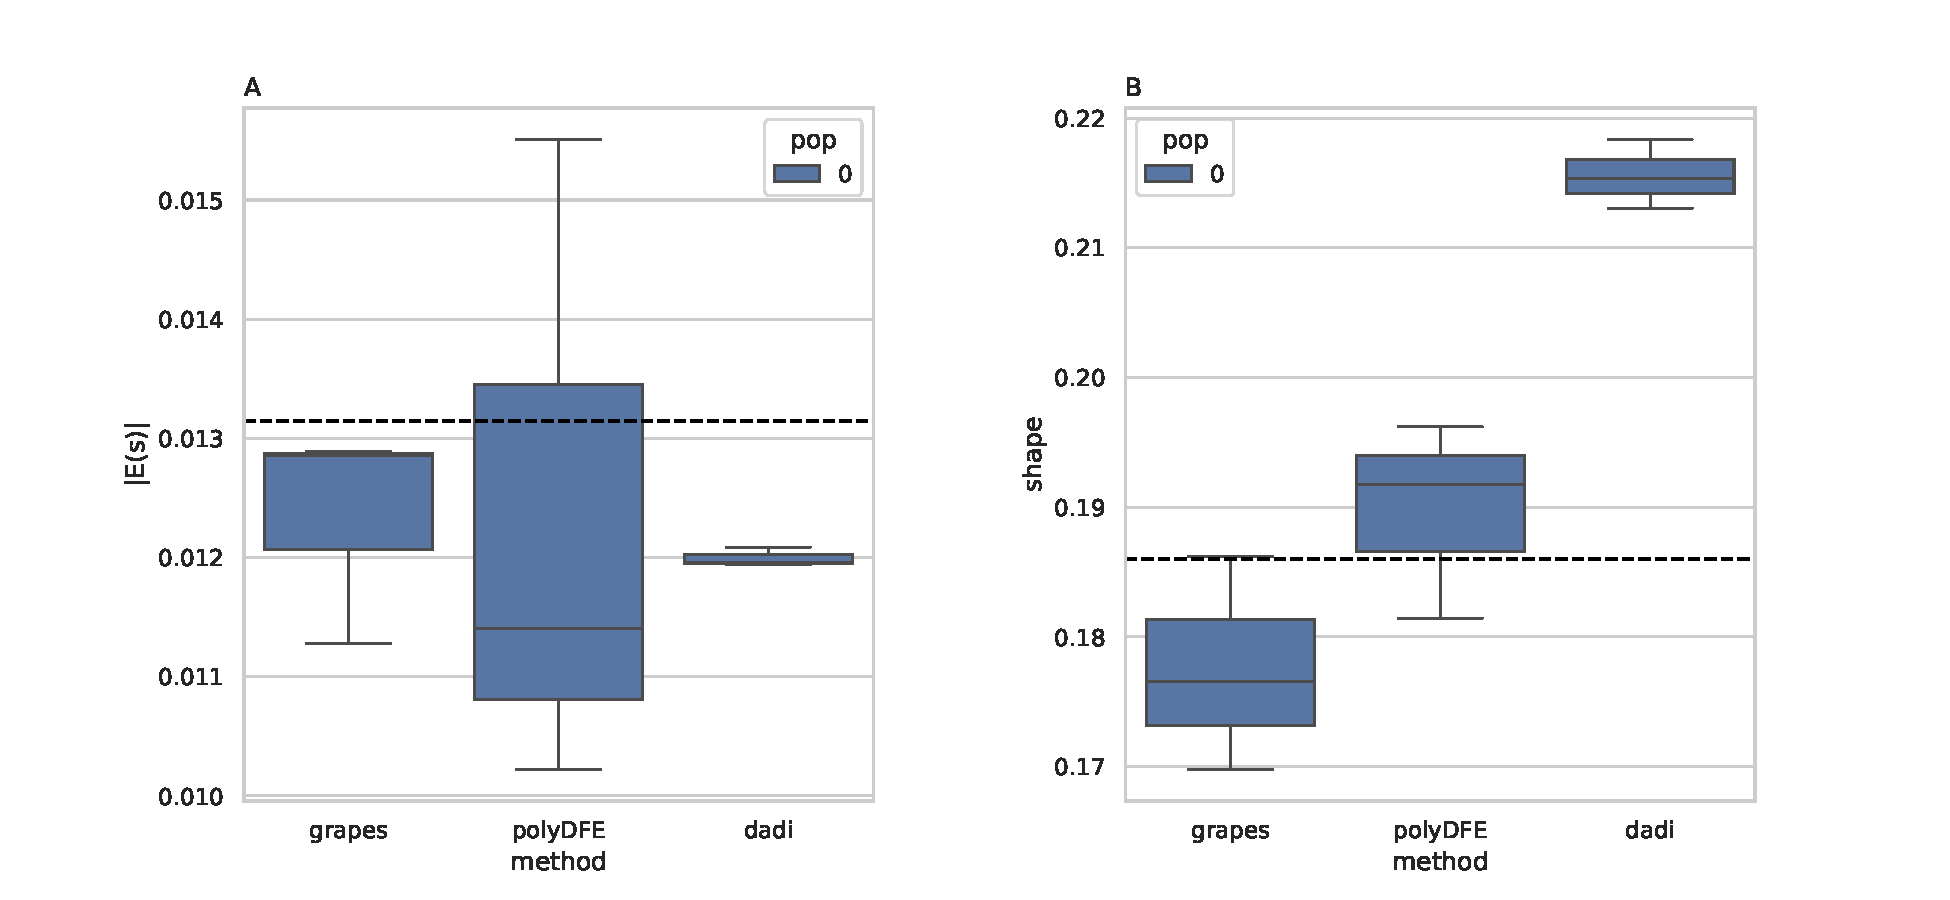
\includegraphics[width=\textwidth]{figures/HomSap/Constant/HomSap_Constant_Gamma_K17_ensembl_havana_104_exons_DFE_plot}
    \caption{
    Performance of methods to infer the distribution of fitness effects (DFE) from genetic data.
    Simulations were performed using a human constant size model with a gamma-distributed DFE
    acting on exons parameterized by a mean selection coefficient and a shape parameter. On each row we show the true parameter 
    as a black line, and the estimates as boxplots from replicate simulations. The human model has three extant populations (CEU, CHB, and YRI).
    %DRS-fig: only one population is shown here, but 3 referenced in the legend. Wrong legend or wrong fig?
    %DRS-fig: If it is the right fig, get rid of the pop0 legend inset
    Each row of the figure shows estimates from a different method: 1) dadi \citep{gutenkunst2009inferring}, 2) polyDFE \citep{tataru2020polydfe},  
    3) DFE-alpha \citep{eyre2009estimating}, and 4) GRAPES \citep{galtier2016adaptive}.  
    }
    \label{fig:homsap-dfe.constant}    
\end{figure}

\begin{figure}
    \centering
    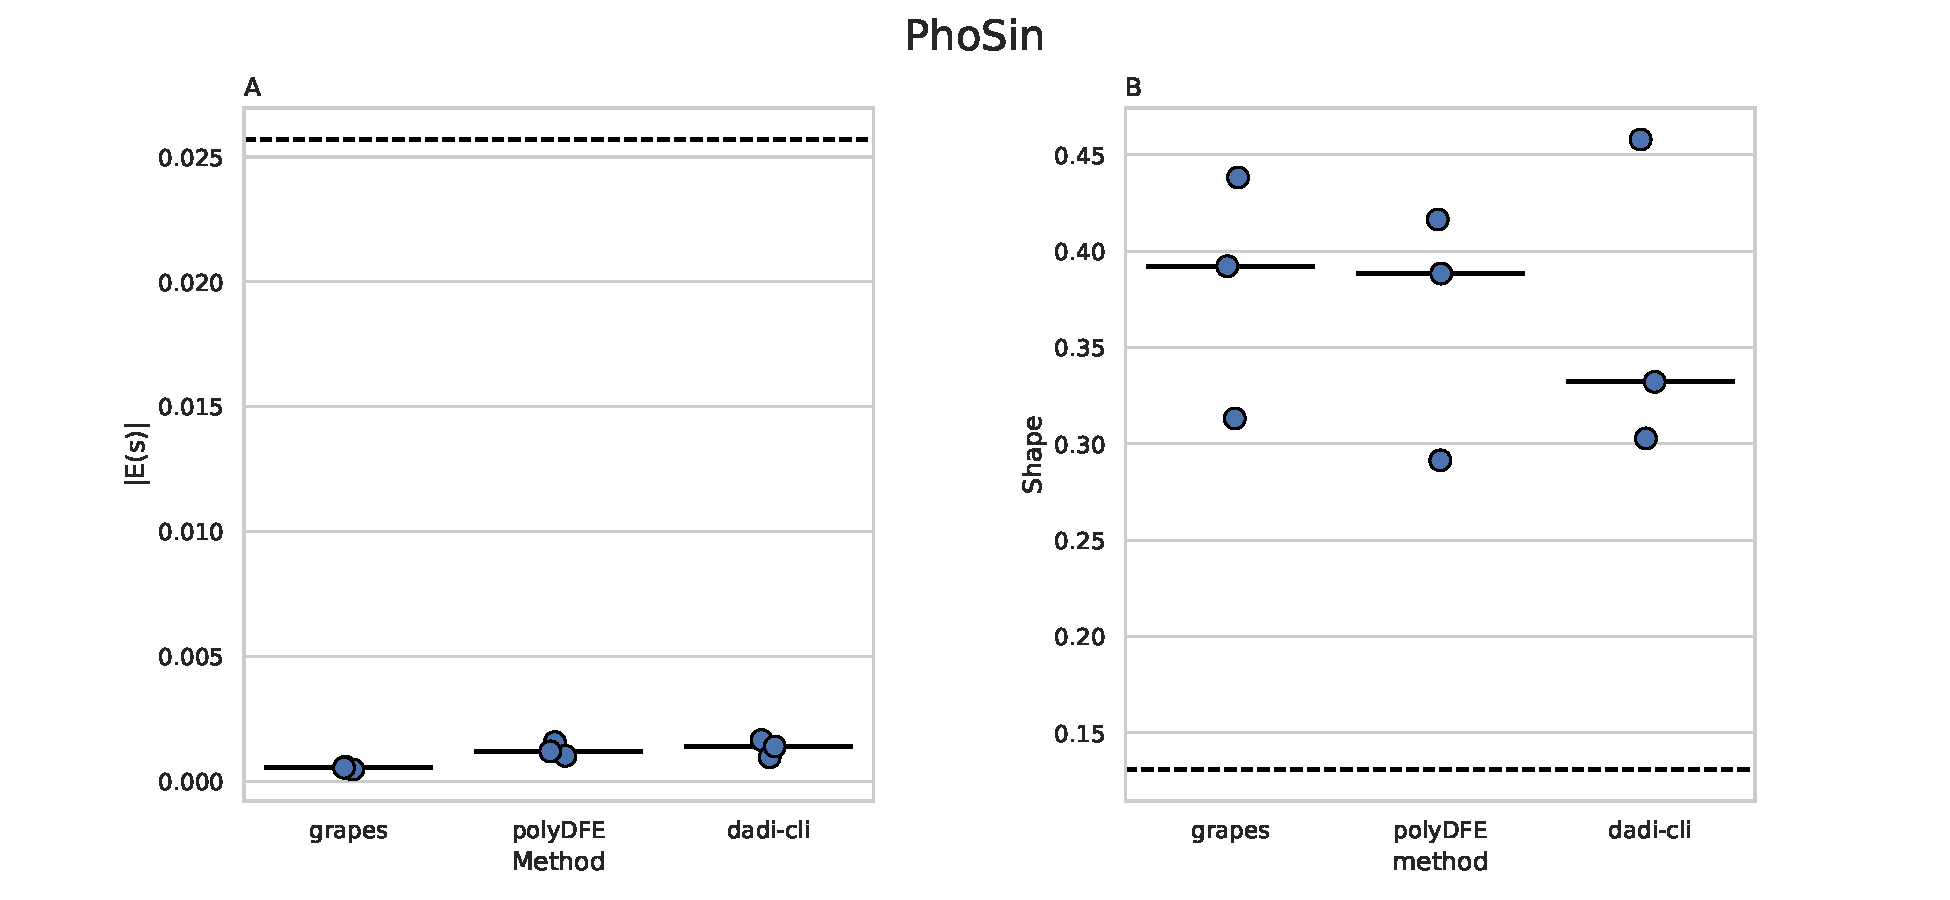
\includegraphics[width=\textwidth]{figures/PhoSin/Constant/PhoSin_Constant_Gamma_R22_Phocoena_sinus.mPhoSin1.pri.110_exons_DFE_plot.pdf}
    \caption{
    \label{fig:vaquita-dfe.constant}
    A comparison of methods for inferring the distribution of fitness effects (DFE) from genetic data.
    Simulations were performed using a model of vaquita porpoise genome under constant population size with a gamma-distributed DFE
    acting on exons parameterized by a mean selection coefficient and a shape parameter. Estimates of the 
    parameters of the DFE are shown in the left ($\lvert E(s) \rvert $) and right hand panels (shape) respectively.
    This vaquita model has a single extant population, and parameter estimates from each
    of the three different methods are shown: 1) GRAPES \citep{galtier2016adaptive}, 2) polyDFE \citep{tataru2020polydfe},
    and 3) dadi \citep{gutenkunst2009inferring}.}
    %DRS-fig: remove the pop 0 legend again
\end{figure}
% DRS-fig: ditch the unnecessary legends from panels A and B. Also, are we deciding which version of panel C to include here? I guess I prefer
% to bottom one but with the legend of the top one (``Original s DFE'' sounds a little clunky).

% constant all site size DFE figure
\begin{figure}[h]
    \centering
    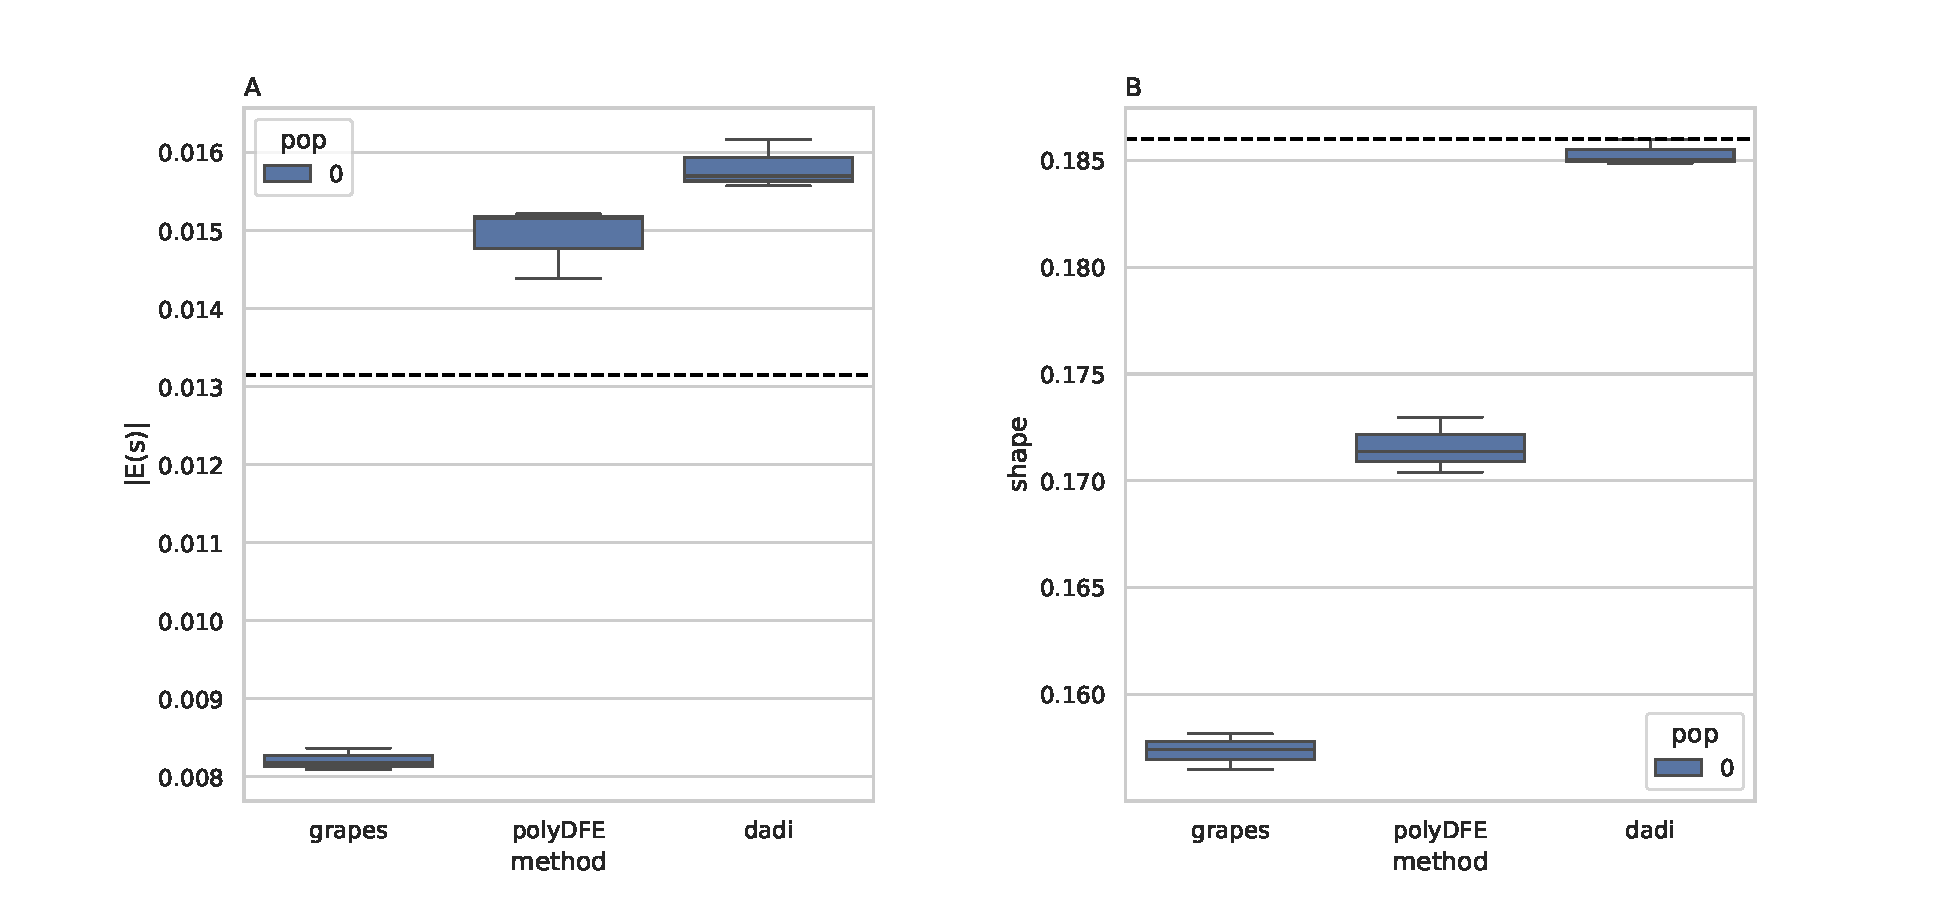
\includegraphics[width=\textwidth]{figures/HomSap/Constant/HomSap_Constant_Gamma_K17_all_sites_DFE_plot}
    \caption{
    \label{fig:homsap-dfe.constant.all_sites}
    Performance of methods to infer the distribution of fitness effects (DFE) from genetic data
    where all sites along the simulated chromosome can experience selected and neutral mutation
    as opposed to exonic regions only.
    }
    %DRS-fig: human? vaquita? need more info in this figure legend, and also get rid of the pop 0 thing again
\end{figure}


\begin{table}[ht]
\centering
\small
\caption{\bf{Performance of DFE methods across the simulation scenarios}. 
Bold rows show the lowest mean absolute error (MAE) for the two DFE parameters
for each species.}
\begin{tabular}{lllrrrrrr}
\toprule
species ID & demography & annotation & \makecell{MAE \\ $E|s|$ \\ dadi} & \makecell{MAE \\ $E|s|$ \\ grapes} & \makecell{MAE \\ $E|s|$ \\ polyDFE} & \makecell{MAE \\ shape \\ dadi} & \makecell{MAE \\ shape \\ grapes} & \makecell{MAE \\ shape \\ polyDFE} \\
\midrule
HomSap & Constant & all sites & 0.0027 & 0.0049 & \bf{0.0018} & \bf{0.00071} & 0.029 & 0.014 \\
HomSap & Constant & exons & 0.0012 & \bf{0.00081} & 0.0023 & 0.030 & 0.0086 & \bf{0.0068} \\
HomSap & OOA 5R19 & all sites & 0.012 & 0.0079 & \bf{0.0074} & \bf{0.027} & 0.055 & 0.035 \\
HomSap & OOA 5R19 & exons & 0.014 & \bf{0.0049} & 0.0072 & 0.031 & 0.051 & \bf{0.024} \\
PhoSin & Constant & all sites & 0.024 & \bf{0.024} & 0.024 & 0.21 & 0.24 & \bf{0.19} \\
PhoSin & Constant & exons & 0.024 & \bf{0.024} & 0.024 & \bf{0.23} & 0.25 & 0.23 \\
PhoSin & Vaquita2Epoch 1R22 & all sites & 0.024 & \bf{0.023} & 0.024 & 0.20 & 0.23 & \bf{0.18} \\
PhoSin & Vaquita2Epoch 1R22 & exons & 0.024 & \bf{0.023} & 0.024 & \bf{0.18} & 0.23 & 0.21 \\
\bottomrule
\end{tabular}
\label{tab:dfe_table}
\end{table}


% roc curves for sweeps
\begin{figure}
    \centering
    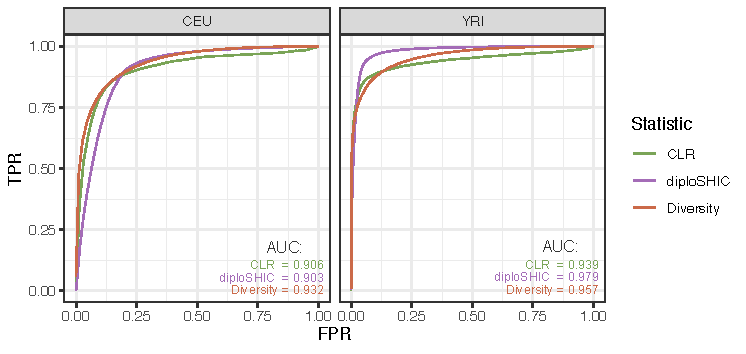
\includegraphics[width=0.8 \textwidth]{figures/sweeps/roc_neutral_null.pdf}
    \caption{
    \label{fig:roc-curves}
    Receiver operating characteristic (ROC) curves for the three methods for detecting sweeps.
    False positive rates were established using neutral simulations that contained no sweeps
    but were conditioned on the same population history as the CEU and YRI samples.
    }
    %DRS-fig: can we include AUCs here?
\end{figure}


%sweep power vs exon density
\begin{figure}
    \centering
    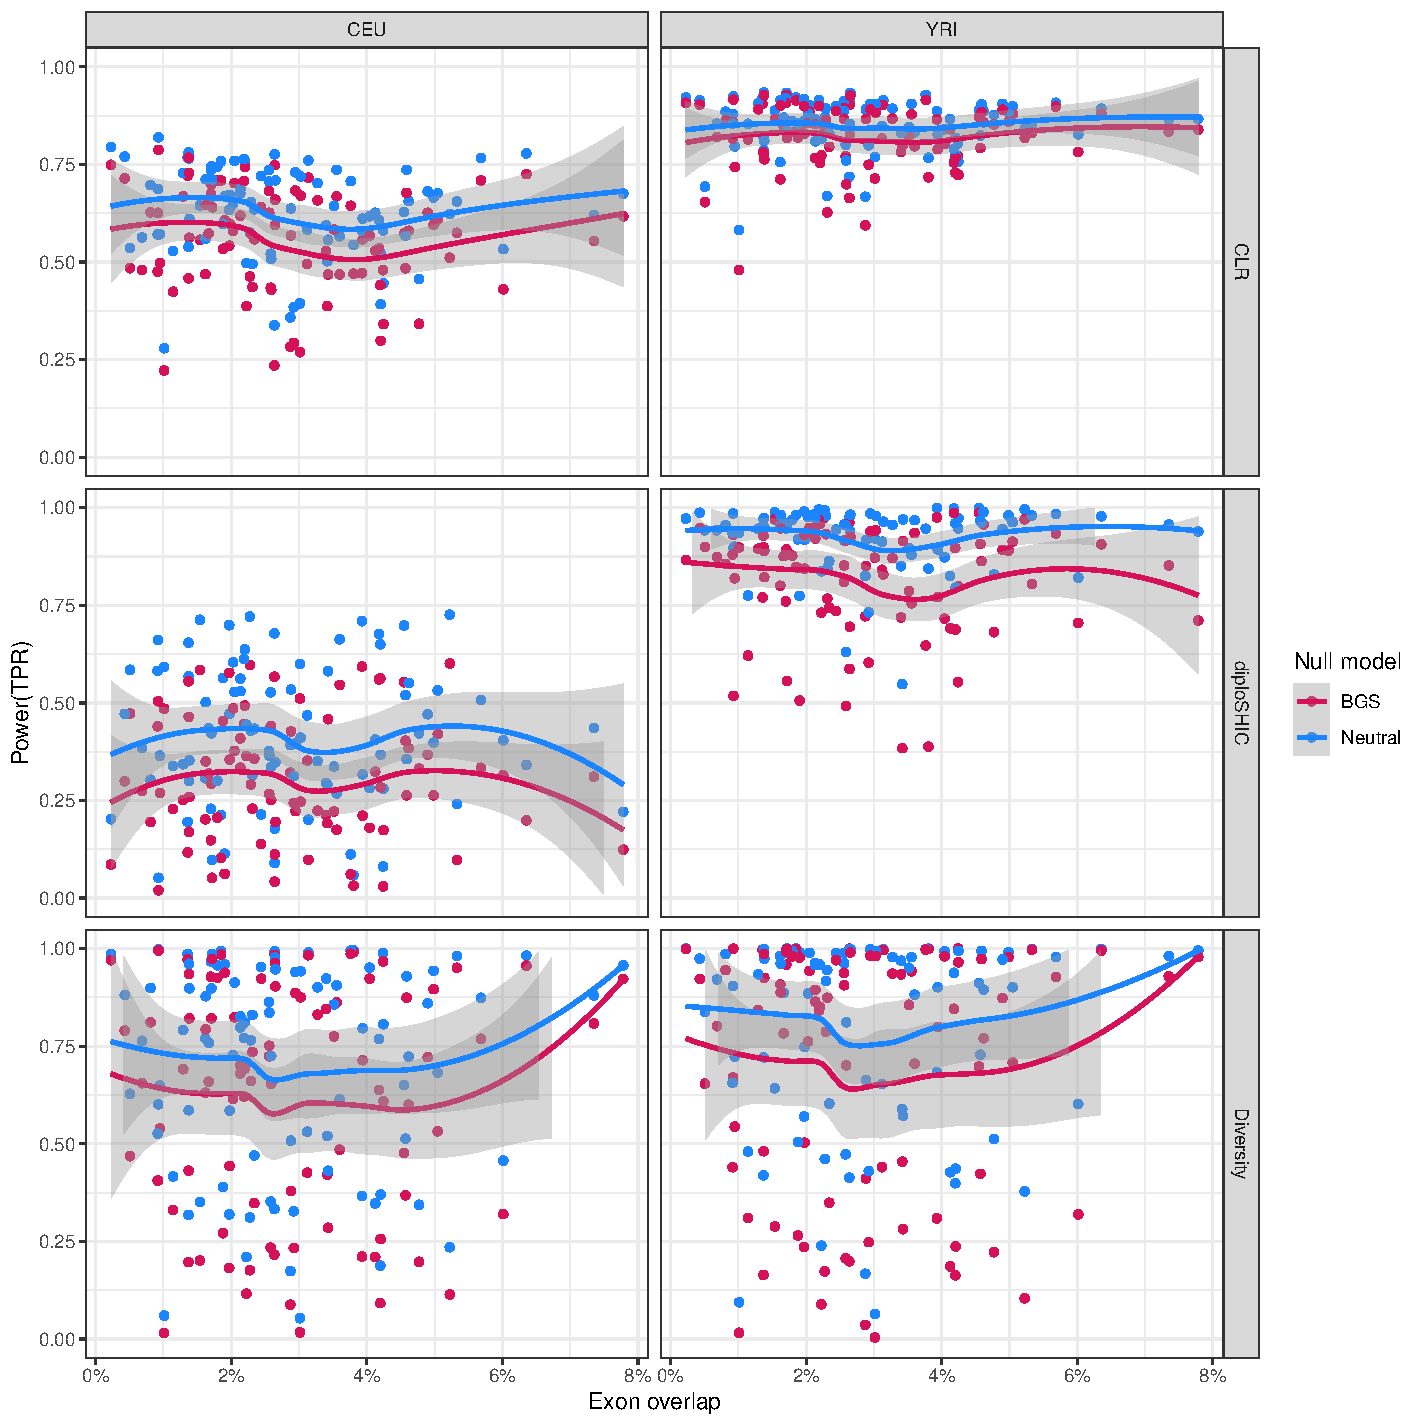
\includegraphics[width=0.8 \textwidth]{figures/sweeps/relationship_power_exon.pdf}
    \caption{
    Power to detect selective sweeps at 100 locations along human chromosome 1 under a three-population out-of-Africa model \citep{gutenkunst2009inferring}  
    with and without purifying selection as a function of local exon density.
    Simulations are as described in Figure \ref{fig:chr1_power}.
    Each panel shows the results of simulations with purifying selection acting on exons (red; labelled BGS)
    and without purifying selection (blue; labelled Neutral).
    True positive rate is shown for these methods for the CEU and YRI samples (left and right respectively).
    Points represent the power at each location and trend lines along with 95\% confidence intervals are shown fit to those points.
    }
    \label{fig:power-exon}
\end{figure}


\stopsupplement
\end{document}
